\documentclass{article}
\usepackage{/Users/jay/LaTeX/cs}
\usepackage{/Users/jay/LaTeX/matlab}

\newcommand{\hmwkClass}{Digital Image Processing, Spring 2018}
\newcommand{\hmwkTitle}{Homework 1}
\newcommand{\hmwkDueDate}{March 28, 2018}
\newcommand{\tb}{\textbf}

\begin{document}

\thispagestyle{empty}
\section*{\hmwkClass \\
    \normalsize{\hmwkTitle} \\
    \normalsize{DUE DATE: \hmwkDueDate}
}

\hfill{Student ID: B03902129 \, Department: CSIE \, Name: Peng-Yu Chen}

% ------ %
% README %
% ------ %
\subsection*{README}

To run my program, simply type \tb{README} in the Command Window of MATLAB application, then it'll run all .m files and output the .raw images.

\begin{lstlisting}[caption = {README.m}]
    % DIP Homework Assignment #1 
    % March 28, 2018
    % Name: Jay Chen
    % ID #: B03902129 
    % email: b03902129@ntu.edu.tw
    
    %#########################################################################
    % Add path first
    %#########################################################################
    
    disp('Add path "./warmup", "./prob1", "./prob2" and "./readwriter"');
    addpath('./warmup');
    addpath('./prob1');
    addpath('./prob2');
    
    disp('Make a parent folder "./outputs"');
    mkdir . outputs
    
    %######################################################################### 
    % WARM-UP: SIMPLE MANIPULATIONS                                           
    % Implementation 1: Convert color image(I1) -> gray-level image(gray)     
    % Implementation 2: Perform diagonal flipping, I1 -> B                    
    % M-files: warmup.m   
    % Usage: run warmup
    % Output: B.raw
    %#########################################################################
    
    fprintf('----------------------------------------\n');
    fprintf('Running "warmup"\n----------------------------------------\n');
    warmup();
    
    %######################################################################### 
    % Problem 1: IMAGE ENHANCEMENT                                            
    % Implementation 1: Decrease the brightness, I2 -> D                      
    % Implementation 2: Plot the histograms of I2 and D
    % Implementation 3: Perform histogram equalization, D -> H
    % Implementation 4: Perform local histogram equalization, D -> L
    % Implementation 5: Plot the histograms of H and L
    % Implementation 6: Perform the log transform, inverse log transform 
    %                   and power-law transform
    % M-files: prob1.m, plotHist.m, histEq.m, localhist.m and trans.m
    % Usage: run prob1 to call other .m files
    % Outputs: D.raw, H.raw and L.raw
    % Parameters:
    %       * Local Histogram Equalization: window size = 3, 5, 7, ..., 255
    %       * Log Transformation: c = 5, 15, 25, ..., 85
    %       * Inverse Log Transformation: c = 1, 2, 3, ..., 9
    %       * Power-Law Transformation: p = 0.2, 0.4, 0.6, ..., 3.0
    %#########################################################################
    
    fprintf('----------------------------------------\n');
    fprintf('Running "prob1"\n----------------------------------------\n');
    prob1();
    
    %######################################################################### 
    % Problem 2: NOISE REMOVAL                                            
    % Implementation 1: Generate Gaussian noise image, I3 -> G1 / G2         
    % Implementation 2: Generate salt-and-pepper noise image, I3 -> S1 / S2
    % Implementation 3: Design Low Pass Filter, G1 -> RG
    % Implementation 4: Design Median Filter, S1 -> RS
    % Implementation 5: Computer PSNR
    % Implementation 6: Remove the wrinkles
    % M-files: prob2.m, addGaussianNoise.m, addSaltAndPepper.m, lowPassFilter.m
    %          squareMedianFilter.m, crossMedianFilter.m, PSNR.m and 
    %          removeWrinkle.m
    % Usage: run prob2 to call other .m files
    % Output: None
    % Parameters:
    %       * 3 x 3 Low Pass Filter: b = 1, 2, 3, ..., 30
    %       * n x n Square Median Filter: window size = 3, 5, 7, ..., 15
    %       * n + n - 1 Cross Median Filter: cross size = 3, 5, 7, ..., 15
    %       * Wrinkle remover: threshold = 3
    %                          crossMedianFilter with cross size = 15
    %#########################################################################
    
    fprintf('----------------------------------------\n');
    fprintf('Running "prob2"\n----------------------------------------\n');
    prob2();    
\end{lstlisting}

\newpage
% ----------------------------- %
% WARM-UP: SIMPLE MANIPULATIONS %
% ----------------------------- %
\subsection*{WARM-UP: SIMPLE MANIPULATIONS}

Please convert the given color image $I_1$ as shown in Fig.1 to a gray-level one. Please also perform diagonal flipping on it and output the result as $B$. \\
To get gray-level image, we add Red, Green and Blue colors, then divide them by 3. \\
To perform diagonal flipping, we use \tb{permute} function.

\begin{figure}[!htb]
    \centering
    \begin{subfigure}[b]{0.3\textwidth}
        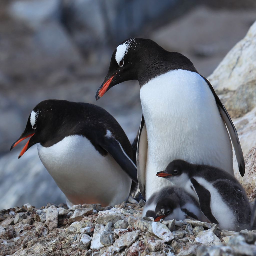
\includegraphics[width=\textwidth]{img/sample1.png}
        \caption{sample1.raw}
    \end{subfigure}
    ~
    \begin{subfigure}[b]{0.3\textwidth}
        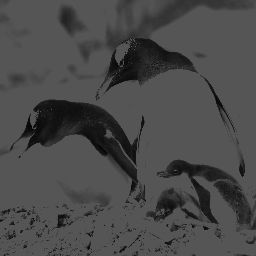
\includegraphics[width=\textwidth]{img/gray.png}
        \caption{gray-level}
    \end{subfigure}
    ~
    \begin{subfigure}[b]{0.3\textwidth}
        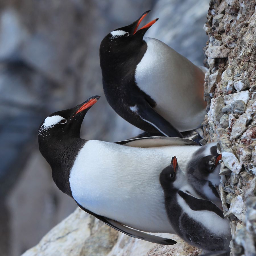
\includegraphics[width=\textwidth]{img/B.png}
        \caption{diagonal flipping}
    \end{subfigure}
    \caption{Penguins}
    \label{Penguins}
\end{figure}

% ---------------------------- %
% PROBLEM 1: IMAGE ENHANCEMENT %
% ---------------------------- %
\subsection*{PROBLEM 1: IMAGE ENHANCEMENT}

Given an image $I_1$ as shown in Fig. 2. Please follow the instructions below to create several new images.

\begin{enumerate}[label=(\alph*)]
    \item Decrease the brightness of $I_2$ by dividing the intensity values by $3$ and output the image as $D$.

    \begin{figure}[!htb]
        \centering
        \begin{subfigure}[b]{0.3\textwidth}
            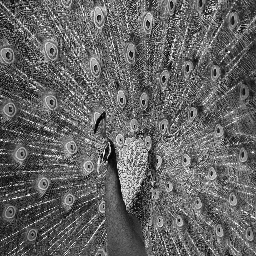
\includegraphics[width=\textwidth]{img/sample2.png}
            \caption{sample2.raw}
        \end{subfigure}
        ~
        \begin{subfigure}[b]{0.3\textwidth}
            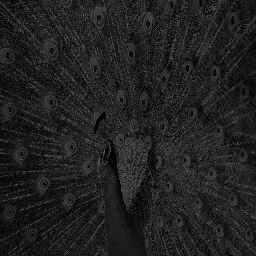
\includegraphics[width=\textwidth]{img/D.png}
            \caption{D.raw}
        \end{subfigure}
        \caption{Darker peacock}
        \label{Darker peacock}
    \end{figure}

    \newpage
    \item Plot the histograms of $I_2$ and $D$.
    
    Since we get $D$ by dividing $I_2$ by $3$, we can see the histogram of $D$ squeezes to the left dramastically.
    
    \begin{figure}[!htb]
        \centering
        \begin{subfigure}[b]{0.45\textwidth}
            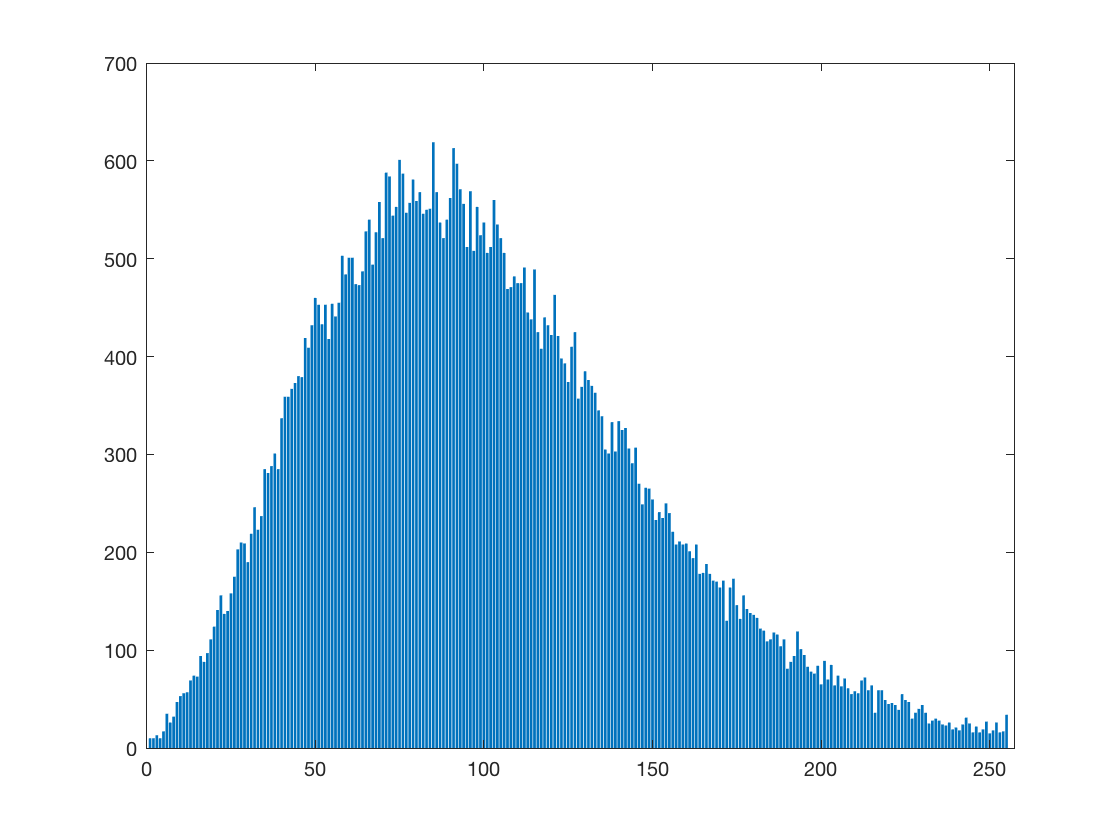
\includegraphics[width=\textwidth]{img/hist_I2.png}
            \caption{histogram of $I_2$}
        \end{subfigure}
        ~
        \begin{subfigure}[b]{0.45\textwidth}
            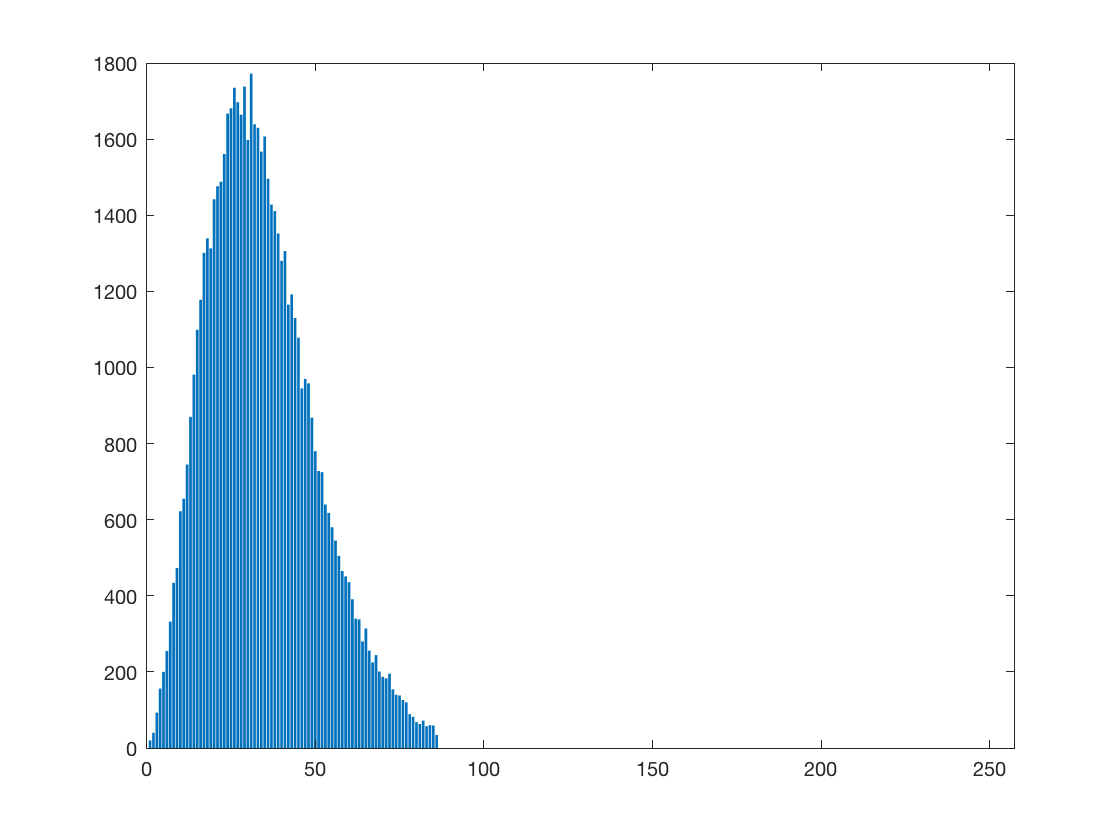
\includegraphics[width=\textwidth]{img/hist_D.png}
            \caption{histogram of $D$}
        \end{subfigure}
        \caption{Histogram comparison after decreasing brightness}
        \label{Histogram comparison after decreasing brightness}
    \end{figure}

    \item Perform histogram equalization on $D$ and output the result as $H$.
    
    \tb{Implementation:}
    let $n_i$ be the number of occurrences of gray level $i$, $L$ be the total number of gray levels in the image (here $L = 256$) and $cdf_x(i) = \sum_{j = 0}^i n_j$.
    
    We can get the general histogram equalization formula is: $$h(i) = \mbox{round}\Big(\frac{cdf(i) - cdf_{\min}}{M \times N - 1} \times (L - 1) \Big).$$
    
    After performing histogram equalization on $D$, the global contrast will increase. The intensities can be better distributed on the histogram.
    
    \begin{figure}[!htb]
        \centering
        \begin{subfigure}[b]{0.3\textwidth}
            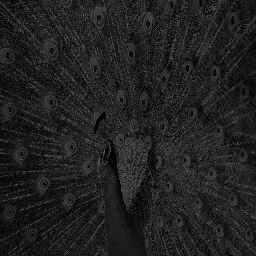
\includegraphics[width=\textwidth]{img/D.png}
            \caption{D.raw}
        \end{subfigure}
        ~
        \begin{subfigure}[b]{0.3\textwidth}
            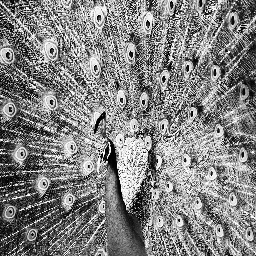
\includegraphics[width=\textwidth]{img/H.png}
            \caption{H.raw}
        \end{subfigure}
        \caption{Histogram equalization comparison}
        \label{Histogram equalization comparison}
    \end{figure}
    
    \newpage
    \item Perform local histogram equalization on image $D$ and output the result as $L$.
    \item Plot the histograms of $H$ and $L$. What's the main difference between local and global histogram equalization?
    
    When the $window.size$ is small ($n \le 7$), the effect is not noticeable. \\
    When the $window.size$ is large ($n > 20$), the contrast become much more readable and it looks similar to H.raw (global histogram equalization).
    
    The main difference is local histogram equalization can distinguish more contrast and can adjust the $window.size$ flexibly.
    
    \begin{figure}[!htb]
        \centering
        \begin{subfigure}[b]{0.3\textwidth}
            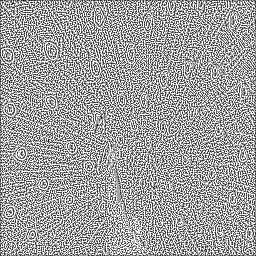
\includegraphics[width=\textwidth]{img/L3.png}
            \caption{$n = 3$}
        \end{subfigure}
        ~
        \begin{subfigure}[b]{0.3\textwidth}
            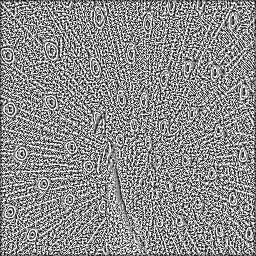
\includegraphics[width=\textwidth]{img/L5.png}
            \caption{$n = 5$}
        \end{subfigure}
        ~
        \begin{subfigure}[b]{0.3\textwidth}
            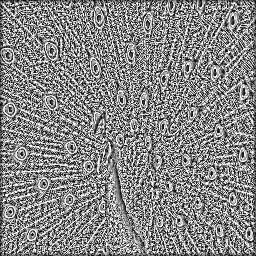
\includegraphics[width=\textwidth]{img/L7.png}
            \caption{$n = 7$}
        \end{subfigure}
        
        % newline
        
        \begin{subfigure}[b]{0.3\textwidth}
            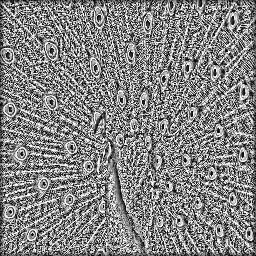
\includegraphics[width=\textwidth]{img/L9.png}
            \caption{$n = 9$}
        \end{subfigure}
        ~
        \begin{subfigure}[b]{0.3\textwidth}
            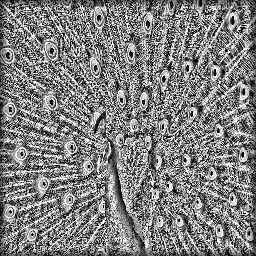
\includegraphics[width=\textwidth]{img/L15.png}
            \caption{$n = 15$}
        \end{subfigure}
        ~
        \begin{subfigure}[b]{0.3\textwidth}
            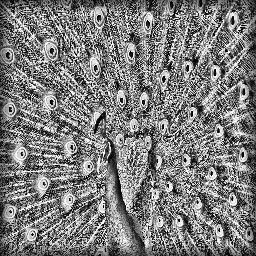
\includegraphics[width=\textwidth]{img/L25.png}
            \caption{$n = 25$}
        \end{subfigure}
        
        % newline
        
        \begin{subfigure}[b]{0.3\textwidth}
            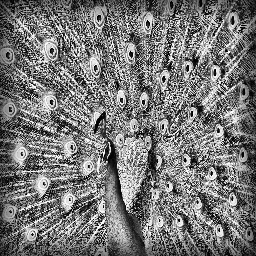
\includegraphics[width=\textwidth]{img/L45.png}
            \caption{$n = 45$}
        \end{subfigure}
        ~
        \begin{subfigure}[b]{0.3\textwidth}
            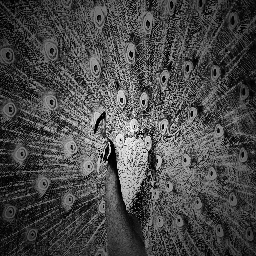
\includegraphics[width=\textwidth]{img/L255.png}
            \caption{$n = 255$}
        \end{subfigure}
        ~
        \begin{subfigure}[b]{0.3\textwidth}
            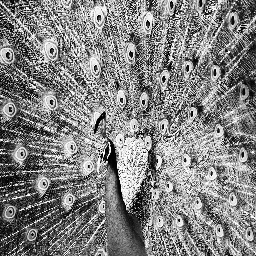
\includegraphics[width=\textwidth]{img/H.png}
            \caption{H.raw}
        \end{subfigure}
        \caption{Local Histogram Equalization with different window sizes $n$}
        \label{Local Histogram Equalization with different window sizes $n$}

    \end{figure}    
    
    \newpage
    When the $window.size = 45$, the histogram distribution is the most uniform, therefore the picture of which is the most distinguishable, too. \\
    When the $window.size = 255$, the histogram left oblique, it means that the picture is darker in that one.

    In this graph, it seems that the global histogram equalization is better than any other local histogram equalizations.

    \begin{figure}[!htb]
        \centering
        \begin{subfigure}[b]{0.3\textwidth}
            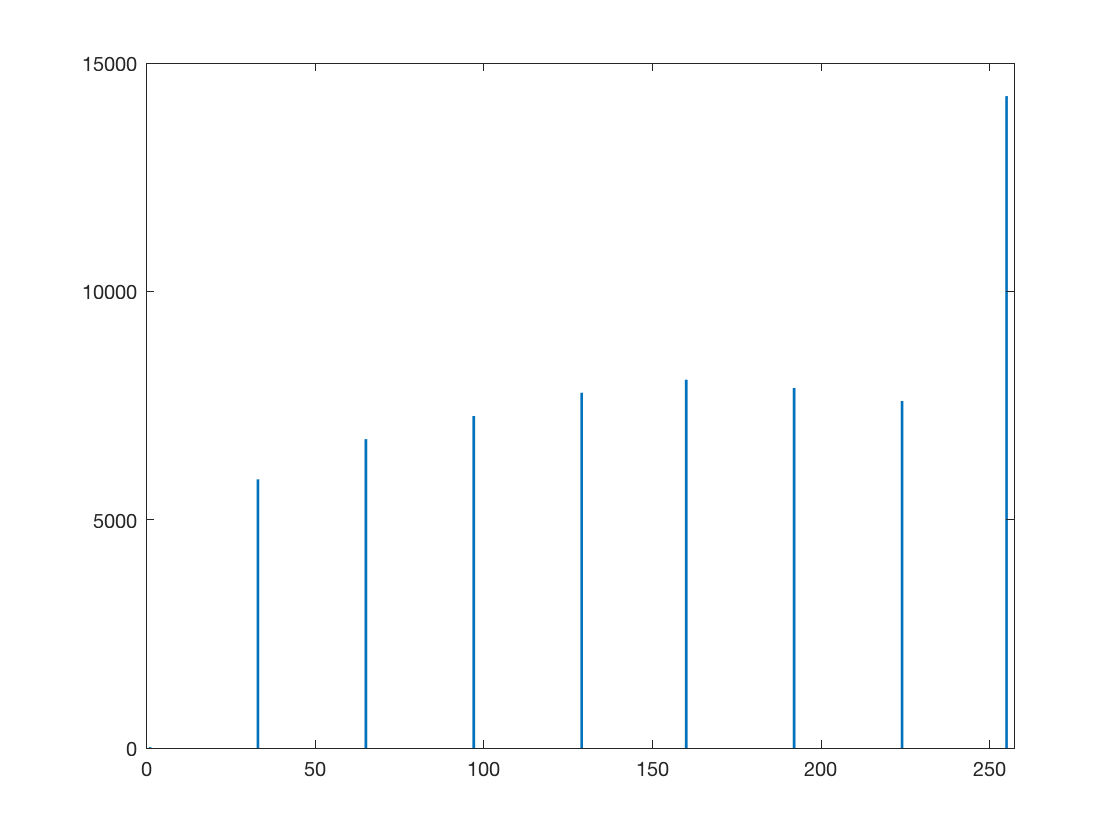
\includegraphics[width=\textwidth]{img/hist_L3.png}
            \caption{$L, n = 3$}
        \end{subfigure}
        ~
        \begin{subfigure}[b]{0.3\textwidth}
            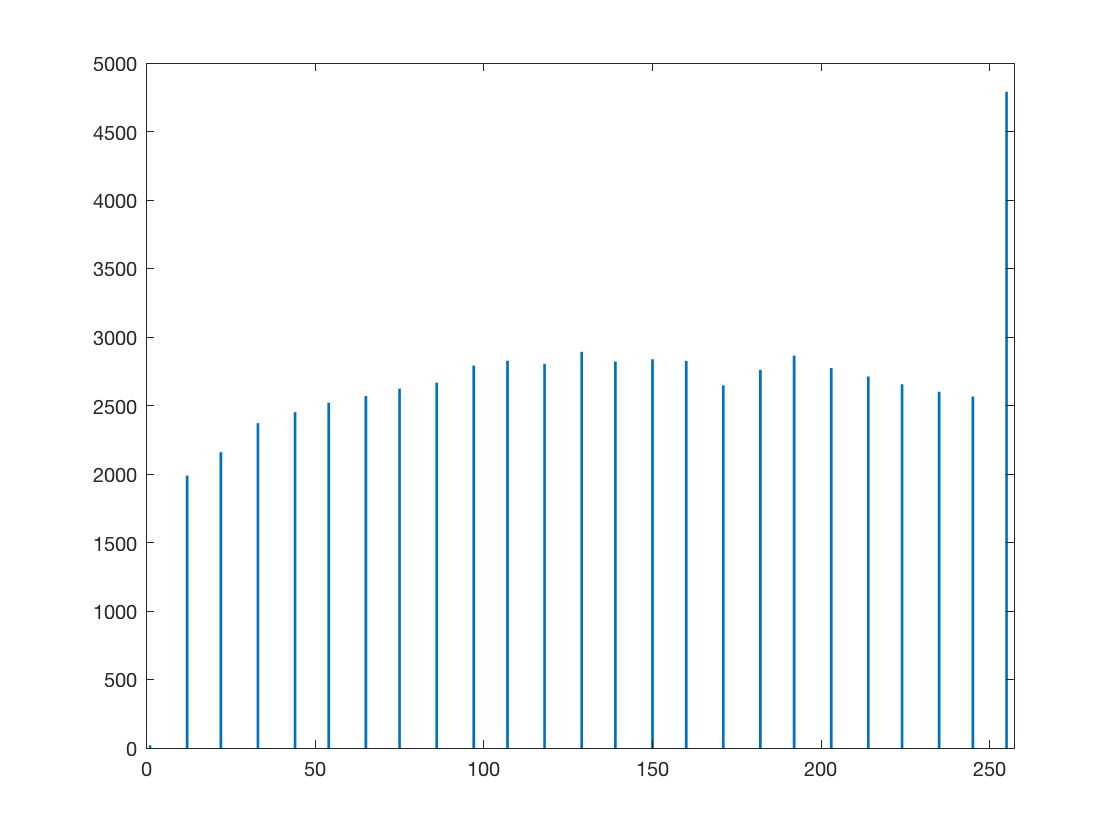
\includegraphics[width=\textwidth]{img/hist_L5.png}
            \caption{$L, n = 5$}
        \end{subfigure}
        ~
        \begin{subfigure}[b]{0.3\textwidth}
            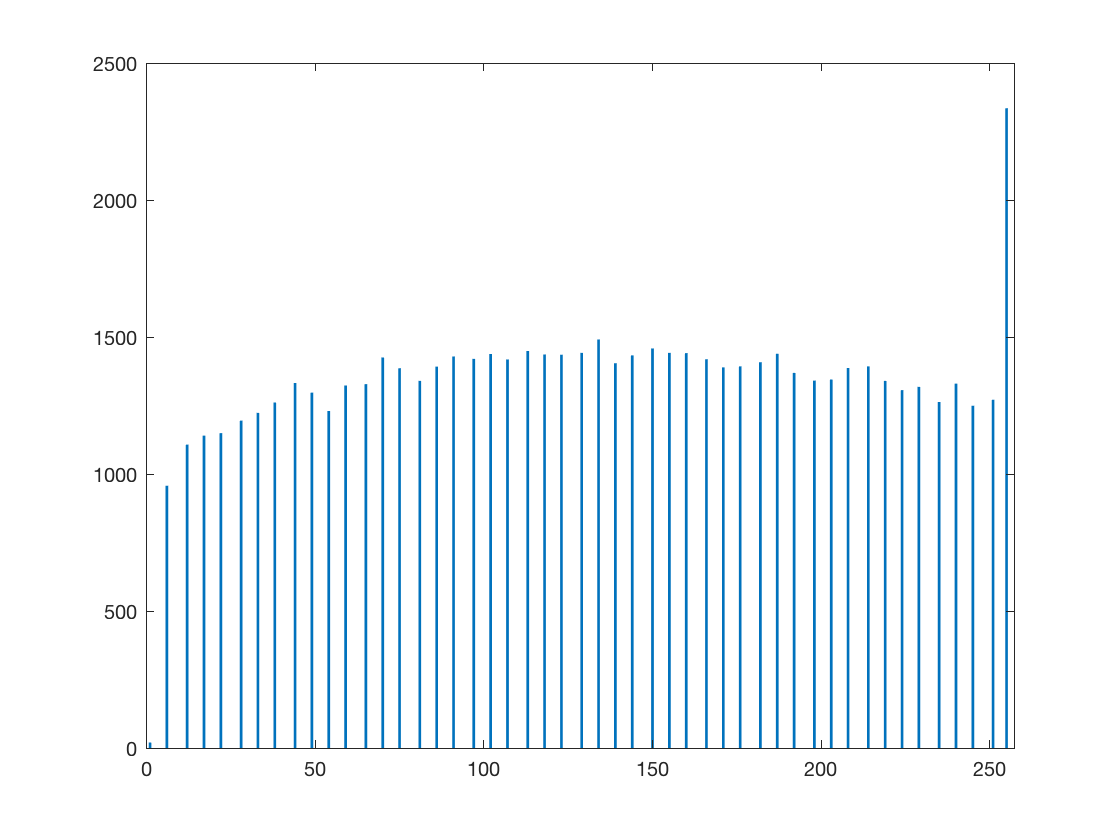
\includegraphics[width=\textwidth]{img/hist_L7.png}
            \caption{$L, n = 7$}
        \end{subfigure}
        
        % newline
        
        \begin{subfigure}[b]{0.3\textwidth}
            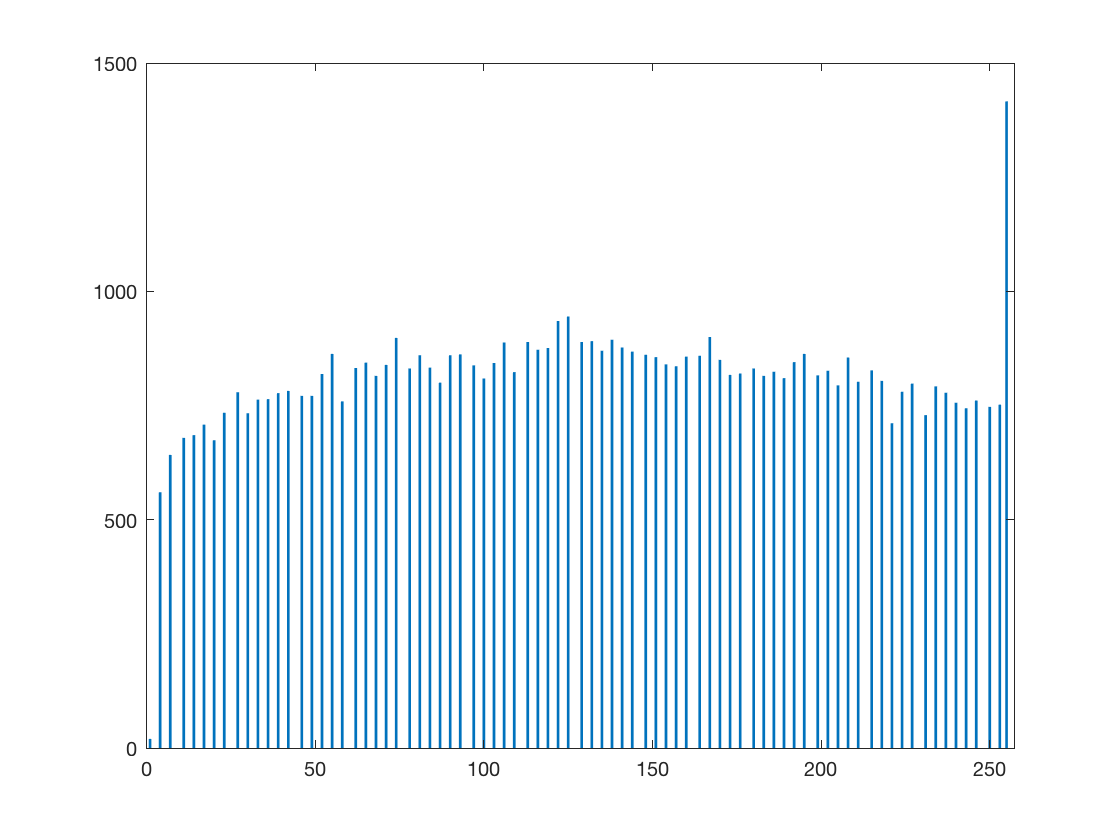
\includegraphics[width=\textwidth]{img/hist_L9.png}
            \caption{$L, n = 9$}
        \end{subfigure}
        ~
        \begin{subfigure}[b]{0.3\textwidth}
            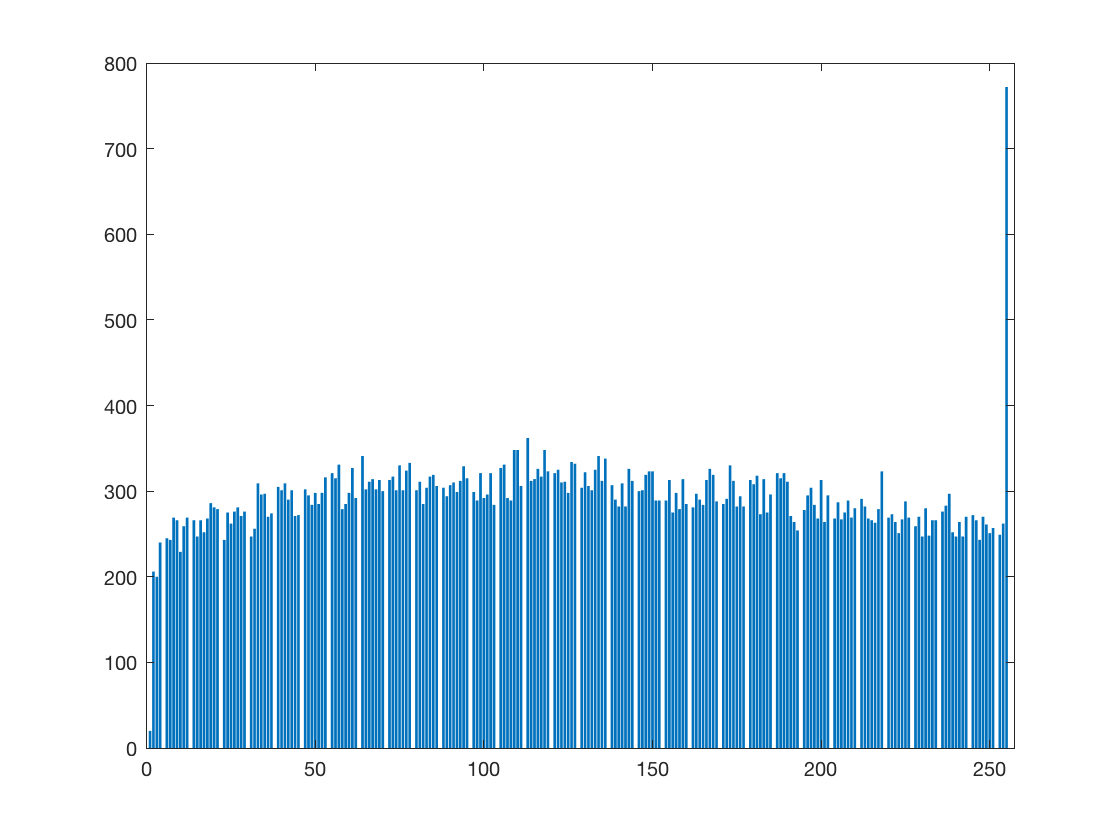
\includegraphics[width=\textwidth]{img/hist_L15.png}
            \caption{$L, n = 15$}
        \end{subfigure}
        ~
        \begin{subfigure}[b]{0.3\textwidth}
            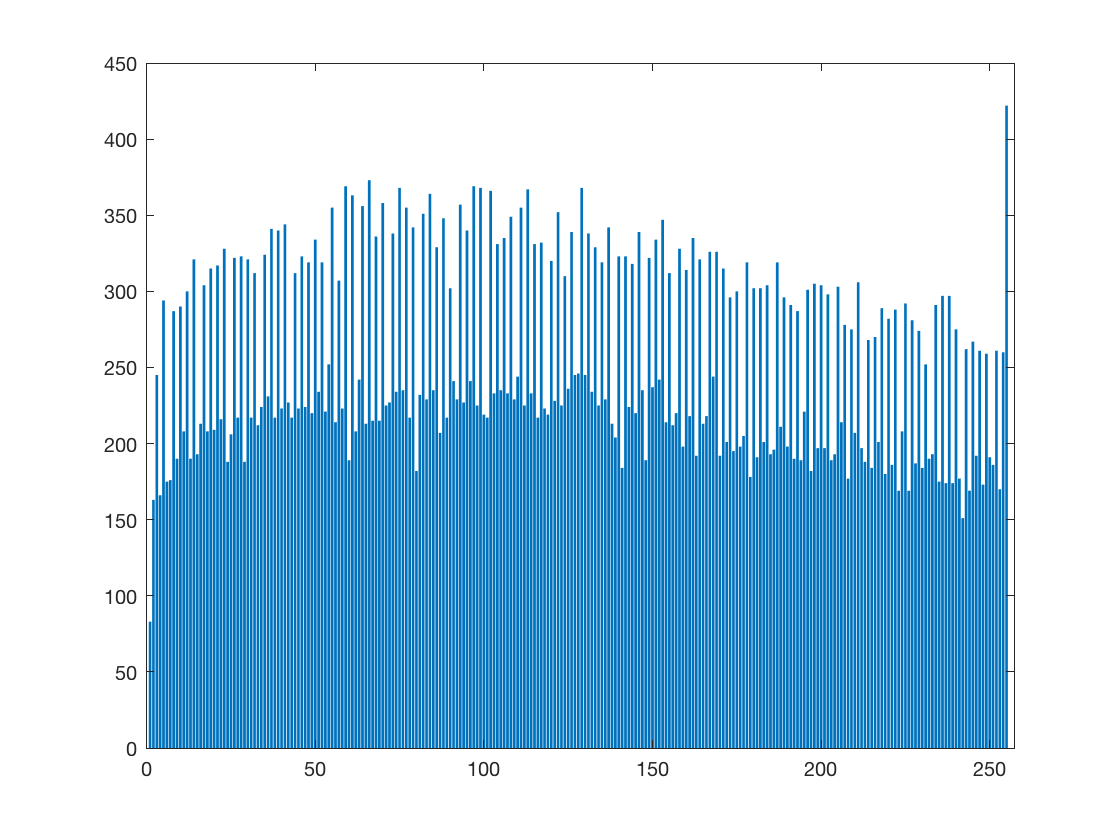
\includegraphics[width=\textwidth]{img/hist_L25.png}
            \caption{$L, n = 25$}
        \end{subfigure}
        
        % newline
        
        \begin{subfigure}[b]{0.3\textwidth}
            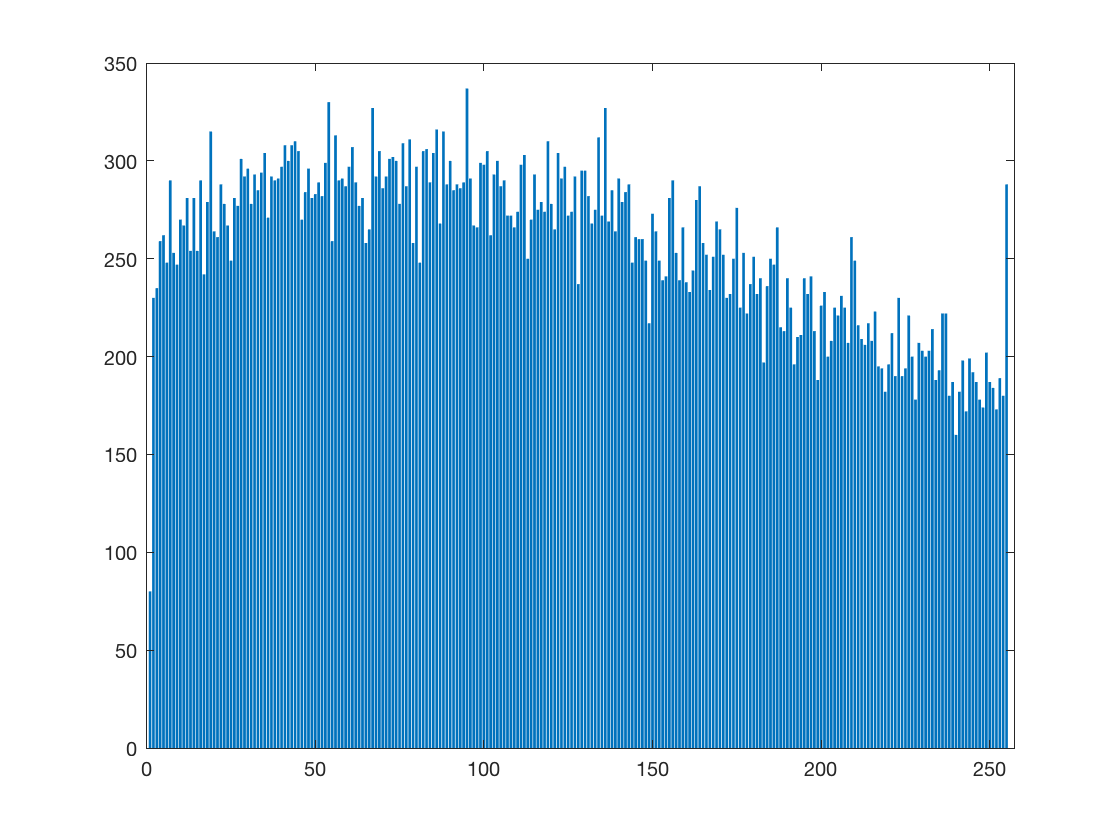
\includegraphics[width=\textwidth]{img/hist_L45.png}
            \caption{$L, n = 45$}
        \end{subfigure}
        ~
        \begin{subfigure}[b]{0.3\textwidth}
            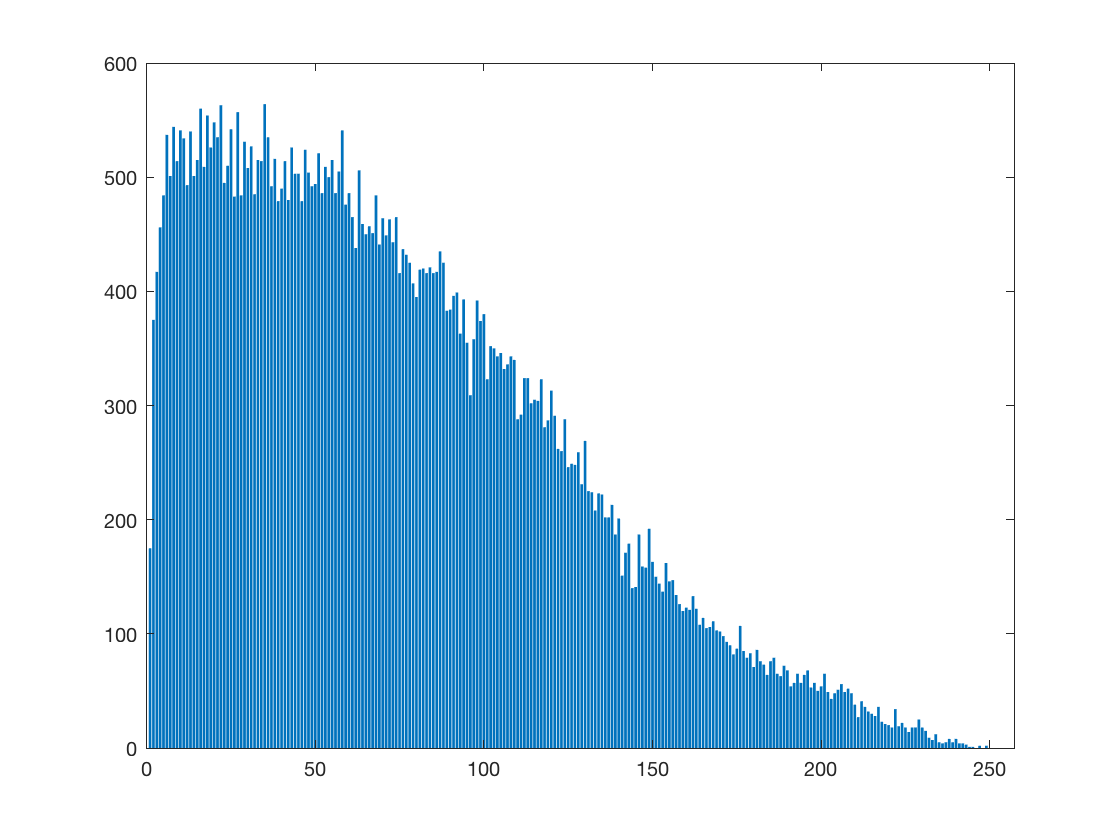
\includegraphics[width=\textwidth]{img/hist_L255.png}
            \caption{$L, n = 255$}
        \end{subfigure}
        ~
        \begin{subfigure}[b]{0.3\textwidth}
            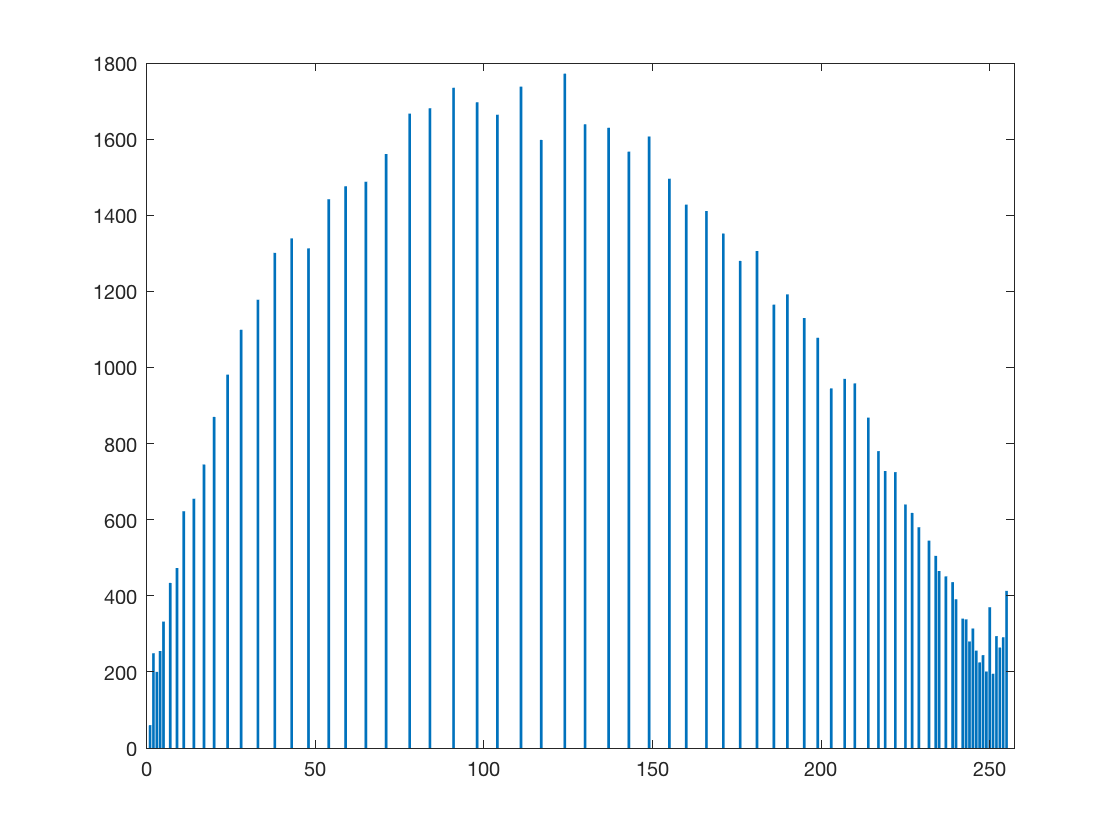
\includegraphics[width=\textwidth]{img/hist_H.png}
            \caption{$H$}
        \end{subfigure}
        \caption{Histograms of $H$ and $L$ with different window sizes $n$}
        \label{Histograms of $H$ and $L$ with different window sizes $n$}
    \end{figure}

    \newpage
    \item Perform the log transform, inverse log transform and power-law transform to enhance image $D$. Please adjust the parameters to obtain the results as best as you can. Show the parameters, resultant images and corresponding histograms. Provide some discussions on the results as well.
    
    \tb{Log Transformation:} $$LT = c \cdot \log(I + 1).$$ 
    
    When $c = (L - 1) / \log L \approx 46$ ($L = 256$), the outcome is better.
    
    \begin{figure}[!htb]
        \centering
        \begin{subfigure}[b]{0.3\textwidth}
            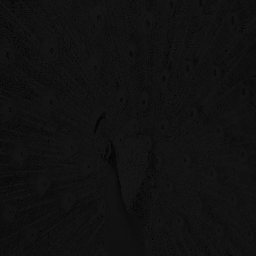
\includegraphics[width=\textwidth]{img/LT5.png}
            \caption{$c = 5$}
        \end{subfigure}
        ~
        \begin{subfigure}[b]{0.3\textwidth}
            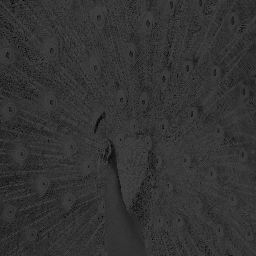
\includegraphics[width=\textwidth]{img/LT15.png}
            \caption{$c = 15$}
        \end{subfigure}
        ~
        \begin{subfigure}[b]{0.3\textwidth}
            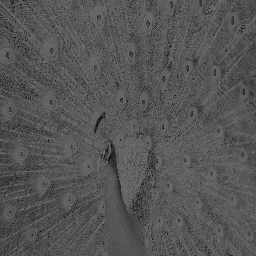
\includegraphics[width=\textwidth]{img/LT25.png}
            \caption{$c = 25$}
        \end{subfigure}
        
        % newline
        
        \begin{subfigure}[b]{0.3\textwidth}
            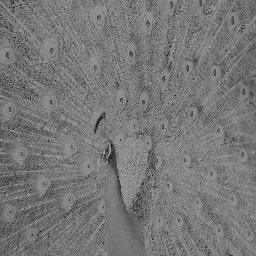
\includegraphics[width=\textwidth]{img/LT35.png}
            \caption{$c = 35$}
        \end{subfigure}
        ~
        \begin{subfigure}[b]{0.3\textwidth}
            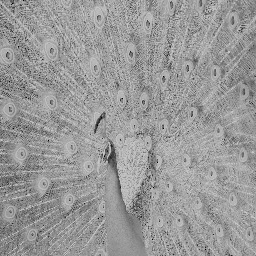
\includegraphics[width=\textwidth]{img/LT45.png}
            \caption{$c = 45$}
        \end{subfigure}
        ~
        \begin{subfigure}[b]{0.3\textwidth}
            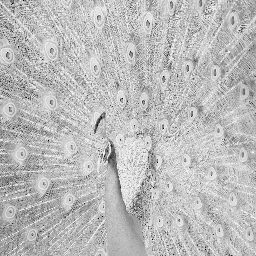
\includegraphics[width=\textwidth]{img/LT55.png}
            \caption{$c = 55$}
        \end{subfigure}
        
        % newline
        
        \begin{subfigure}[b]{0.3\textwidth}
            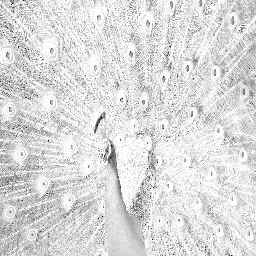
\includegraphics[width=\textwidth]{img/LT65.png}
            \caption{$c = 65$}
        \end{subfigure}
        ~
        \begin{subfigure}[b]{0.3\textwidth}
            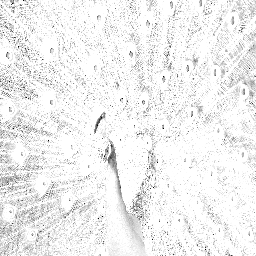
\includegraphics[width=\textwidth]{img/LT75.png}
            \caption{$c = 75$}
        \end{subfigure}
        ~
        \begin{subfigure}[b]{0.3\textwidth}
            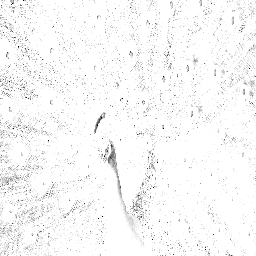
\includegraphics[width=\textwidth]{img/LT85.png}
            \caption{$c = 85$}
        \end{subfigure}
        \caption{Log Transformation with different parameters $c$}
        \label{Log Transformation with different parameters $c$}        
    \end{figure}    
    
    \newpage
    The histogram of log transformation also becomes smoother when $c$ is near $(L - 1) / \log L$ ($L = 256$), i.e., $c$ is between $45$ and $55$, so I think $c \approx 46$ is the best parameter.
    
    \begin{figure}[!htb]
        \centering
        \begin{subfigure}[b]{0.3\textwidth}
            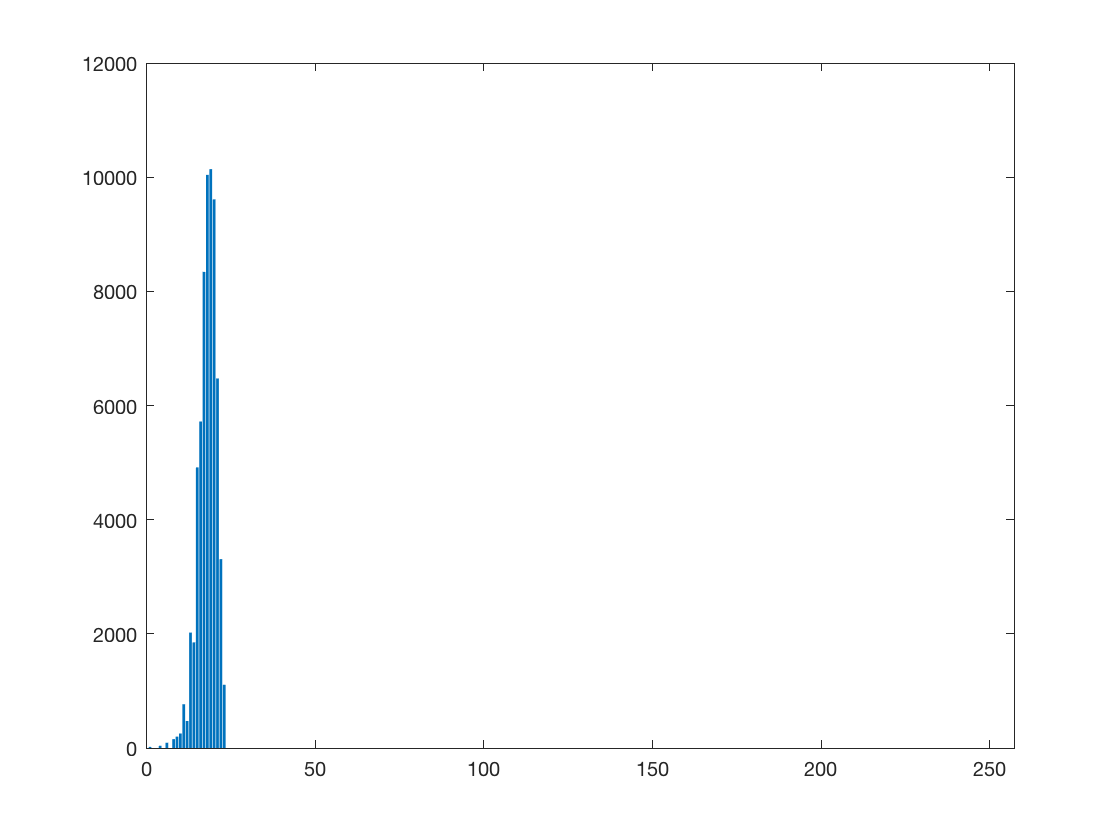
\includegraphics[width=\textwidth]{img/hist_LT5.png}
            \caption{$c = 5$}
        \end{subfigure}
        ~
        \begin{subfigure}[b]{0.3\textwidth}
            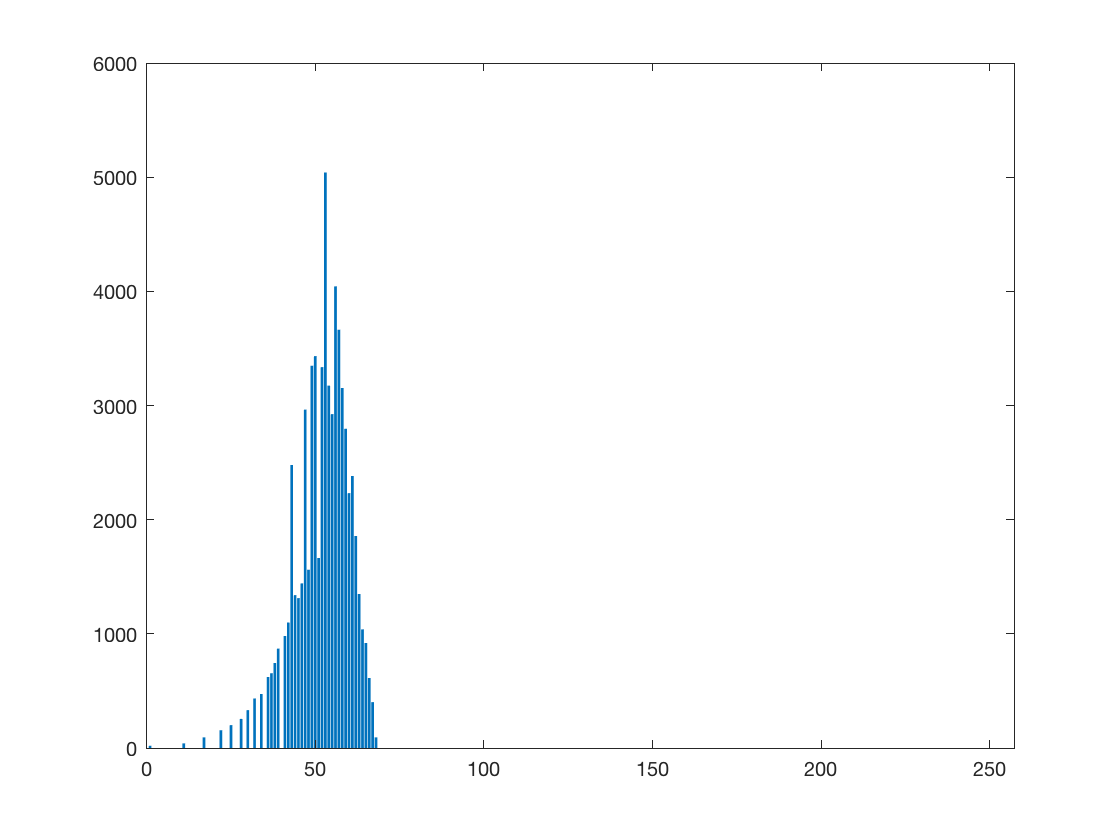
\includegraphics[width=\textwidth]{img/hist_LT15.png}
            \caption{$c = 15$}
        \end{subfigure}
        ~
        \begin{subfigure}[b]{0.3\textwidth}
            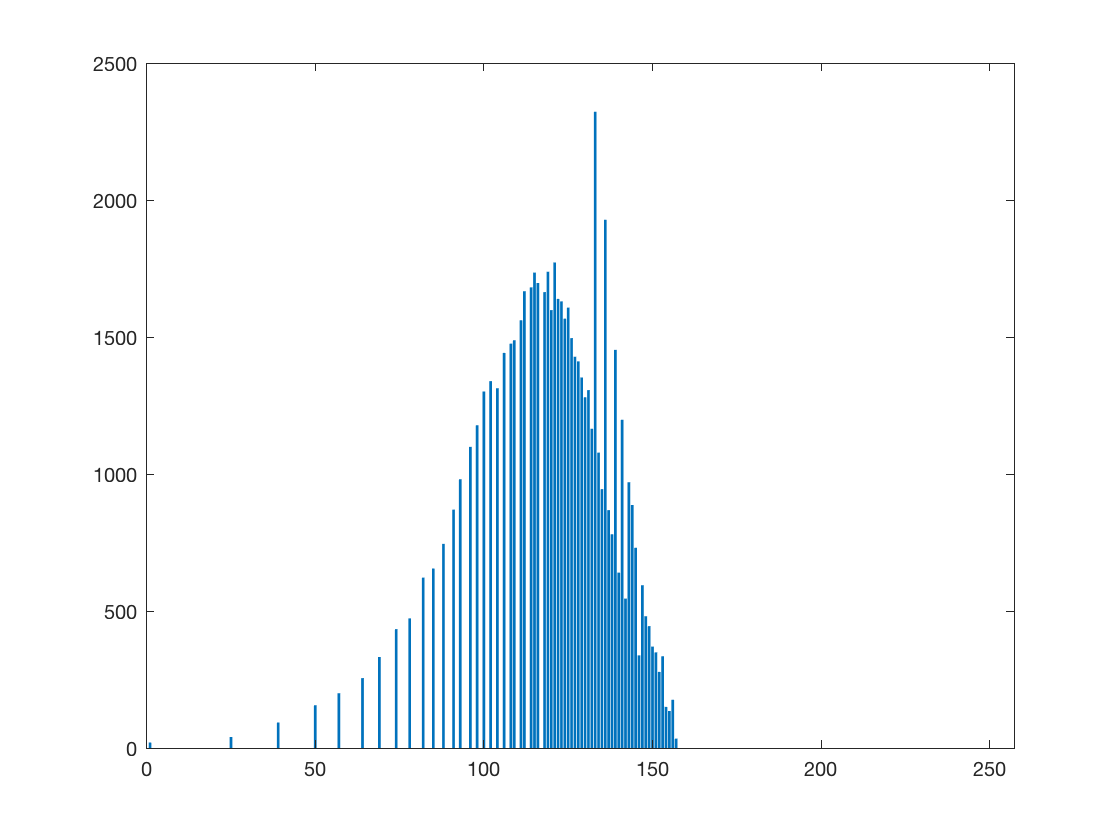
\includegraphics[width=\textwidth]{img/hist_LT25.png}
            \caption{$c = 25$}
        \end{subfigure}
        
        % newline
        
        \begin{subfigure}[b]{0.3\textwidth}
            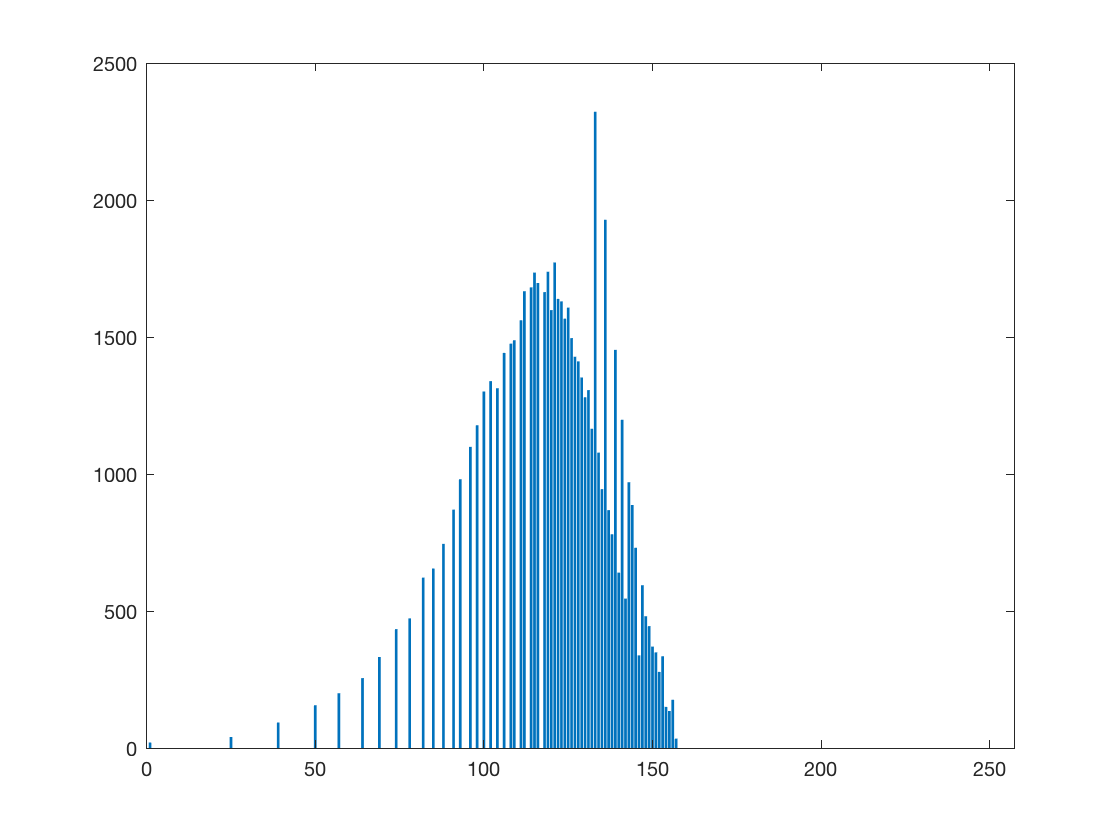
\includegraphics[width=\textwidth]{img/hist_LT35.png}
            \caption{$c = 35$}
        \end{subfigure}
        ~
        \begin{subfigure}[b]{0.3\textwidth}
            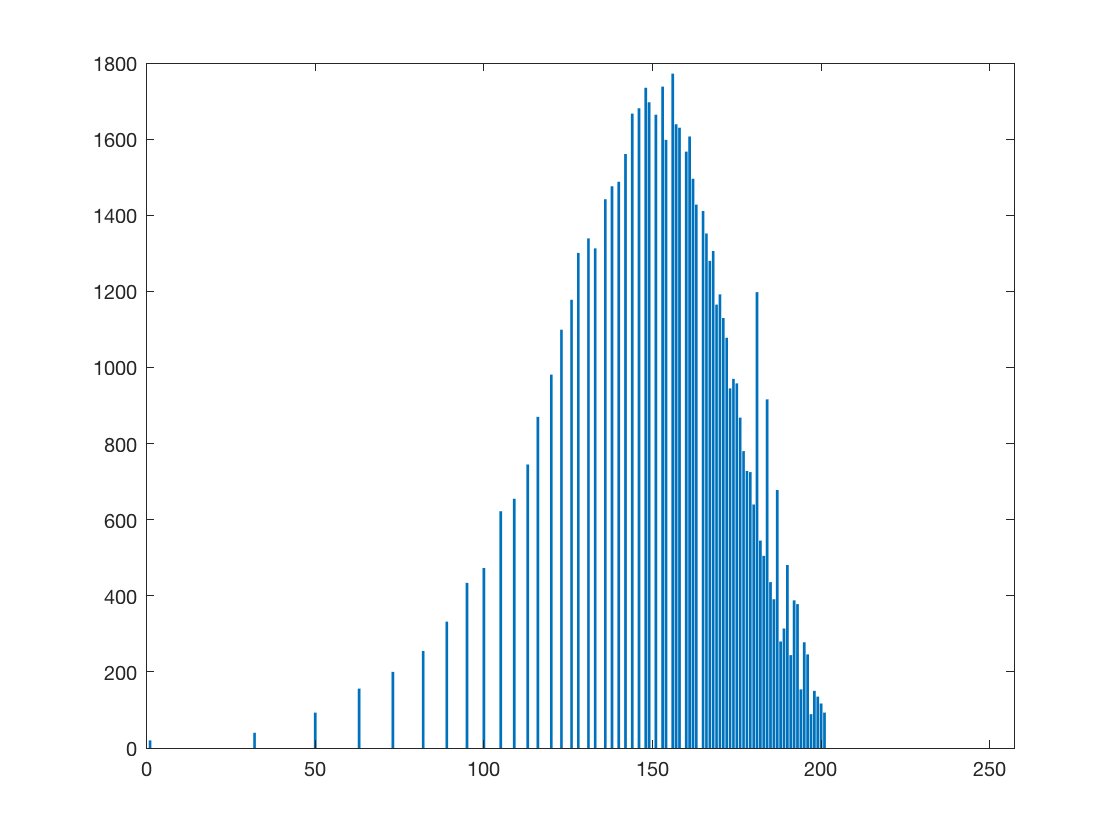
\includegraphics[width=\textwidth]{img/hist_LT45.png}
            \caption{$c = 45$}
        \end{subfigure}
        ~
        \begin{subfigure}[b]{0.3\textwidth}
            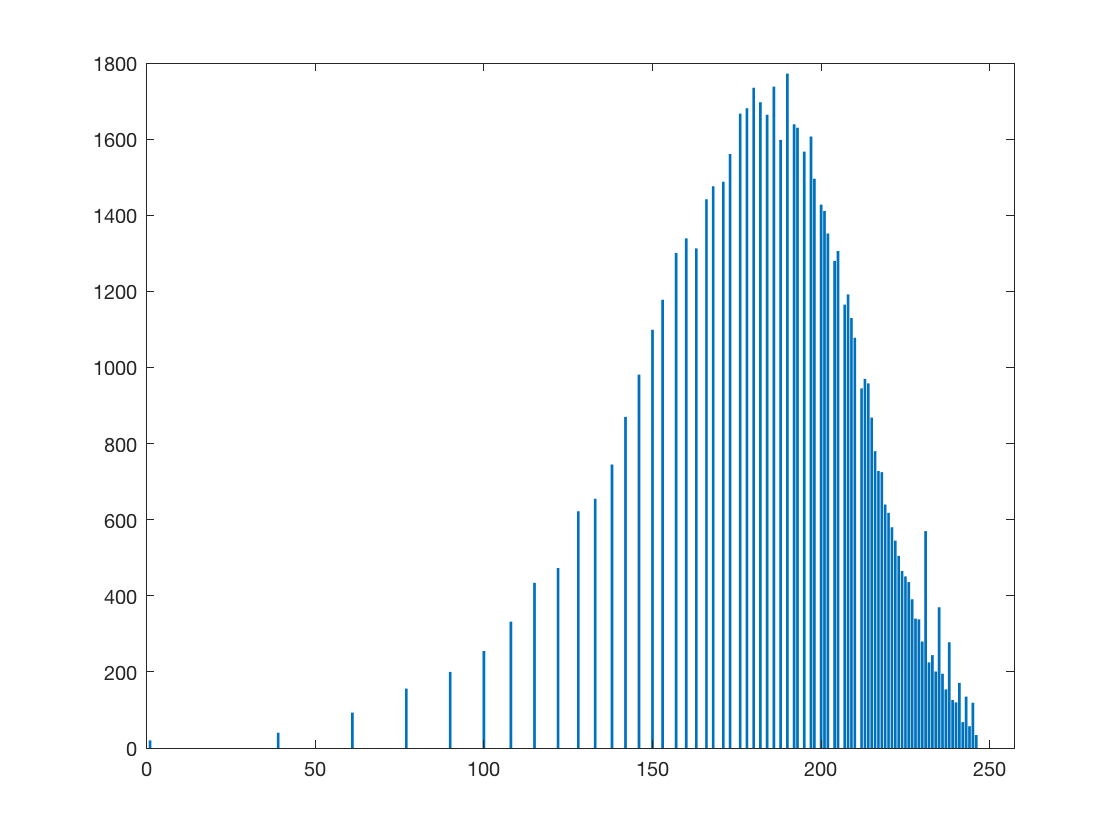
\includegraphics[width=\textwidth]{img/hist_LT55.png}
            \caption{$c = 55$}
        \end{subfigure}
        
        % newline
        
        \begin{subfigure}[b]{0.3\textwidth}
            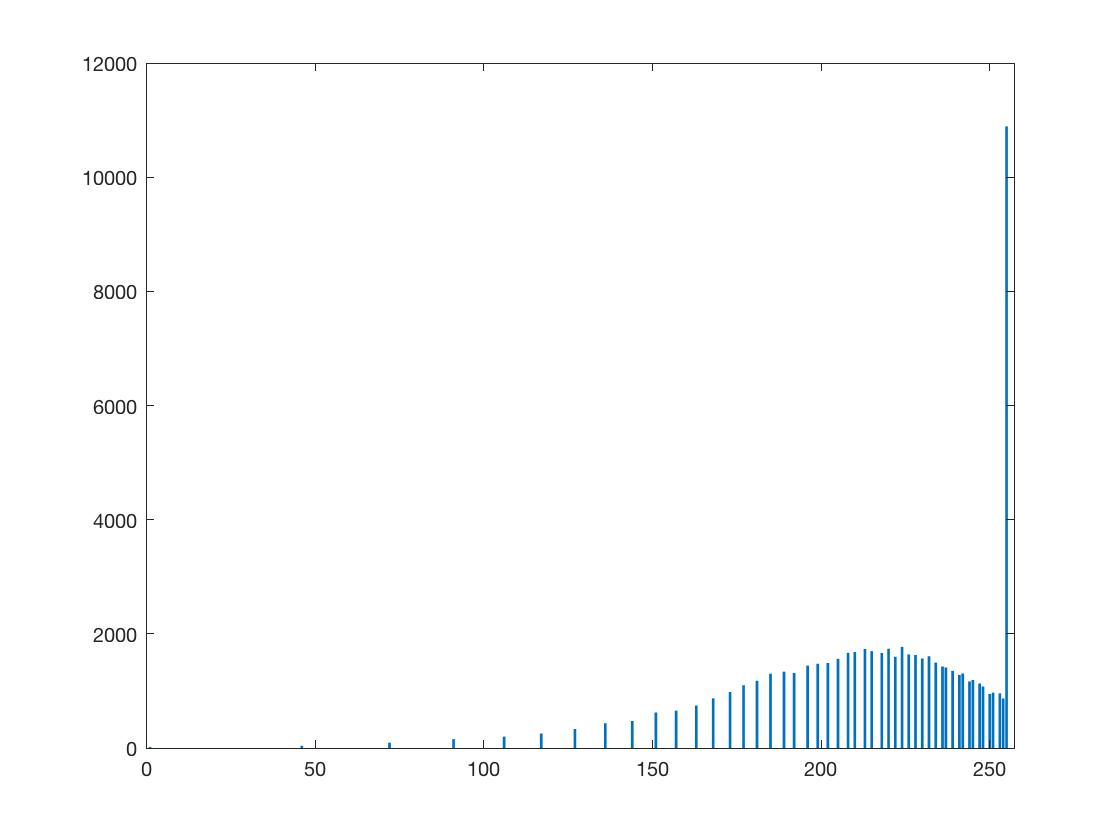
\includegraphics[width=\textwidth]{img/hist_LT65.png}
            \caption{$c = 65$}
        \end{subfigure}
        ~
        \begin{subfigure}[b]{0.3\textwidth}
            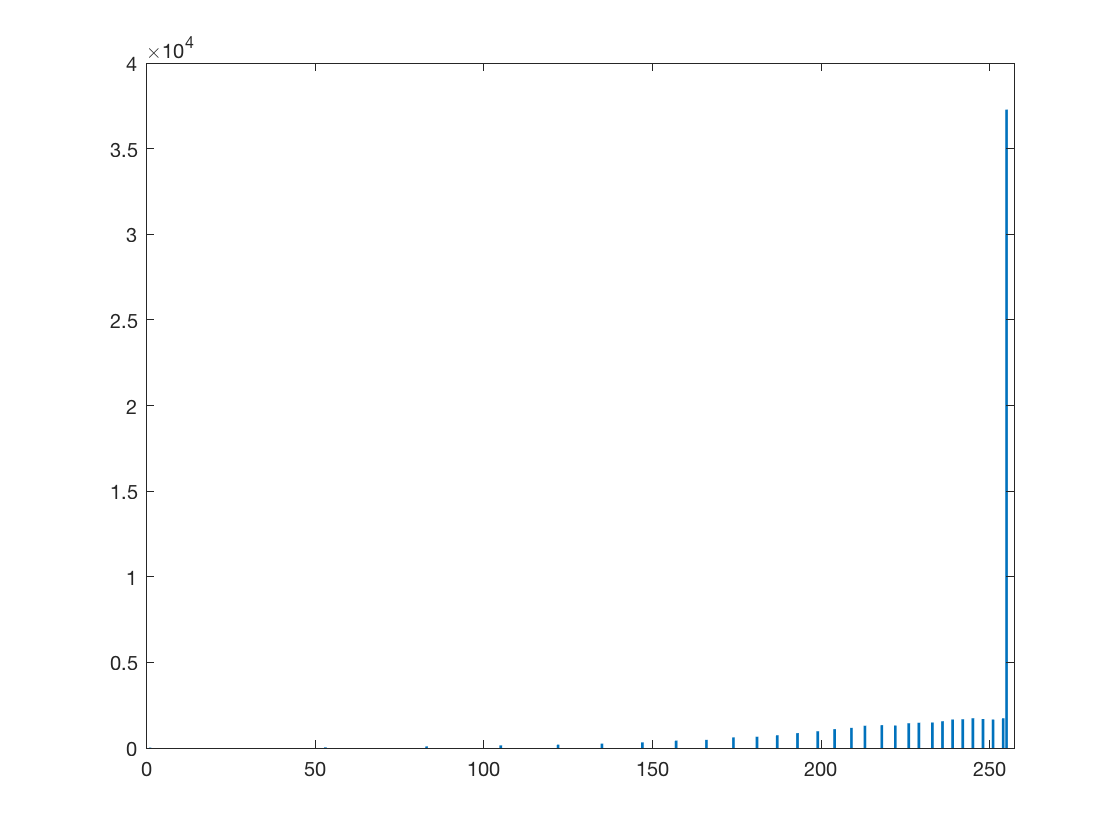
\includegraphics[width=\textwidth]{img/hist_LT75.png}
            \caption{$c = 75$}
        \end{subfigure}
        ~
        \begin{subfigure}[b]{0.3\textwidth}
            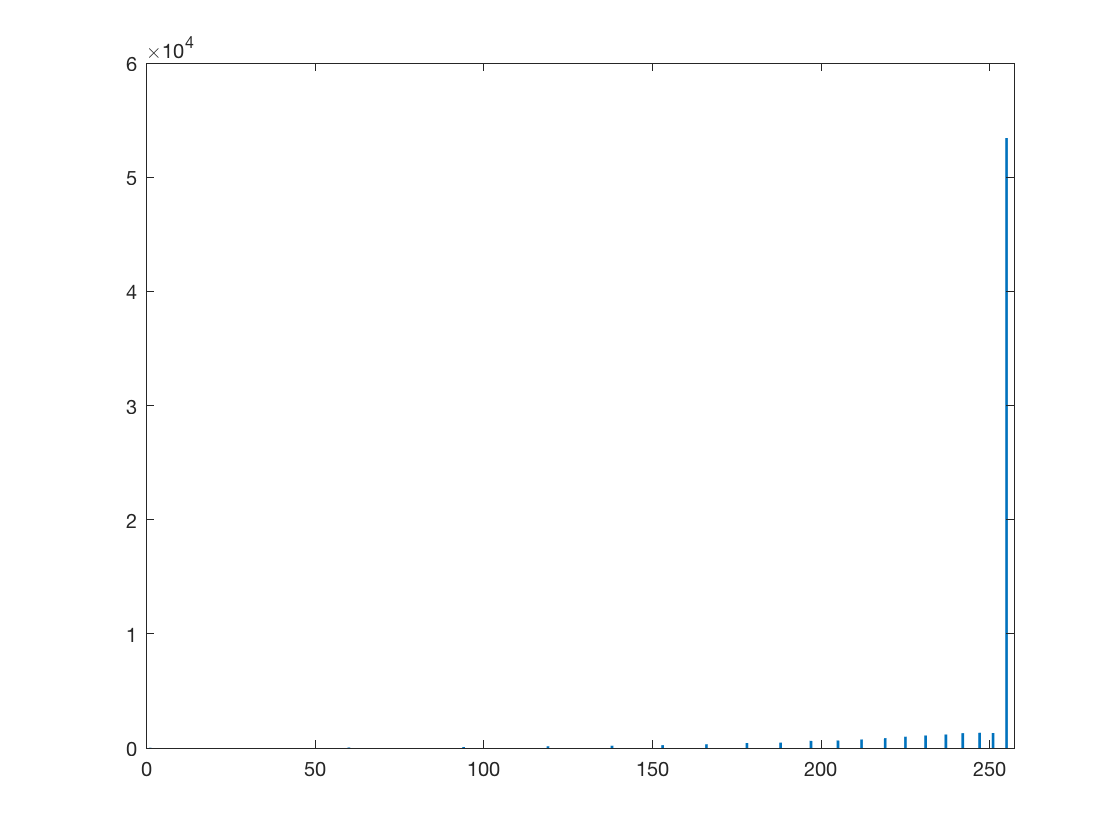
\includegraphics[width=\textwidth]{img/hist_LT85.png}
            \caption{$c = 85$}
        \end{subfigure}
        \caption{Histograms of Log Transformation with different parameters $c$}
        \label{Histograms of Log Transformation with different parameters $c$}        
    \end{figure}
    
    \newpage
    \tb{Inverse Log Transformation:} $$ILT = {(e^I)}^{(1 / c)} - 1.$$ 

    \begin{figure}[!htb]
        \centering
        \begin{subfigure}[b]{0.3\textwidth}
            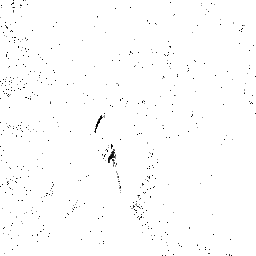
\includegraphics[width=\textwidth]{img/ILT1.png}
            \caption{$c = 1$}
        \end{subfigure}
        ~
        \begin{subfigure}[b]{0.3\textwidth}
            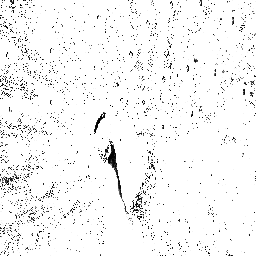
\includegraphics[width=\textwidth]{img/ILT2.png}
            \caption{$c = 2$}
        \end{subfigure}
        ~
        \begin{subfigure}[b]{0.3\textwidth}
            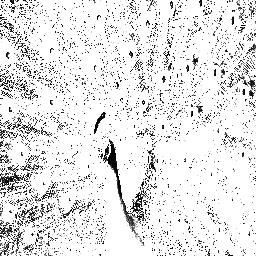
\includegraphics[width=\textwidth]{img/ILT3.png}
            \caption{$c = 3$}
        \end{subfigure}
        
        % newline
        
        \begin{subfigure}[b]{0.3\textwidth}
            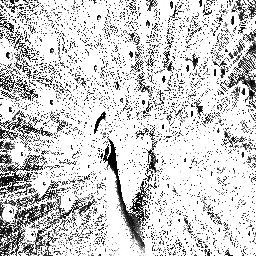
\includegraphics[width=\textwidth]{img/ILT4.png}
            \caption{$c = 4$}
        \end{subfigure}
        ~
        \begin{subfigure}[b]{0.3\textwidth}
            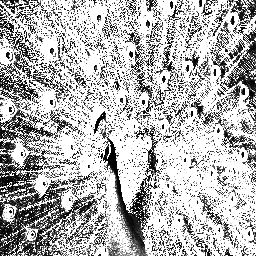
\includegraphics[width=\textwidth]{img/ILT5.png}
            \caption{$c = 5$}
        \end{subfigure}
        ~
        \begin{subfigure}[b]{0.3\textwidth}
            \includegraphics[width=\textwidth]{img/ILT6.png}
            \caption{$c = 6$}
        \end{subfigure}
        
        % newline
        
        \begin{subfigure}[b]{0.3\textwidth}
            \includegraphics[width=\textwidth]{img/ILT7.png}
            \caption{$c = 7$}
        \end{subfigure}
        ~
        \begin{subfigure}[b]{0.3\textwidth}
            \includegraphics[width=\textwidth]{img/ILT8.png}
            \caption{$c = 8$}
        \end{subfigure}
        ~
        \begin{subfigure}[b]{0.3\textwidth}
            \includegraphics[width=\textwidth]{img/ILT9.png}
            \caption{$c = 9$}
        \end{subfigure}
        \caption{Inverse Log Transformation with different parameters $c$}
        \label{Inverse Log Transformation with different parameters $c$}        
    \end{figure}
    
    \newpage
    The histogram of inverse log transformation also becomes smoother when $c$ is between $6$ and $7$, so I think $c \approx 6.5$ is the best parameter.
    \begin{figure}[!htb]
        \centering
        \begin{subfigure}[b]{0.3\textwidth}
            \includegraphics[width=\textwidth]{img/hist_ILT1.png}
            \caption{$c = 1$}
        \end{subfigure}
        ~
        \begin{subfigure}[b]{0.3\textwidth}
            \includegraphics[width=\textwidth]{img/hist_ILT2.png}
            \caption{$c = 2$}
        \end{subfigure}
        ~
        \begin{subfigure}[b]{0.3\textwidth}
            \includegraphics[width=\textwidth]{img/hist_ILT3.png}
            \caption{$c = 3$}
        \end{subfigure}
        
        % newline
        
        \begin{subfigure}[b]{0.3\textwidth}
            \includegraphics[width=\textwidth]{img/hist_ILT4.png}
            \caption{$c = 4$}
        \end{subfigure}
        ~
        \begin{subfigure}[b]{0.3\textwidth}
            \includegraphics[width=\textwidth]{img/hist_ILT5.png}
            \caption{$c = 5$}
        \end{subfigure}
        ~
        \begin{subfigure}[b]{0.3\textwidth}
            \includegraphics[width=\textwidth]{img/hist_ILT6.png}
            \caption{$c = 6$}
        \end{subfigure}
        
        % newline
        
        \begin{subfigure}[b]{0.3\textwidth}
            \includegraphics[width=\textwidth]{img/hist_ILT7.png}
            \caption{$c = 7$}
        \end{subfigure}
        ~
        \begin{subfigure}[b]{0.3\textwidth}
            \includegraphics[width=\textwidth]{img/hist_ILT8.png}
            \caption{$c = 8$}
        \end{subfigure}
        ~
        \begin{subfigure}[b]{0.3\textwidth}
            \includegraphics[width=\textwidth]{img/hist_ILT9.png}
            \caption{$c = 9$}
        \end{subfigure}
        \caption{Histograms of Inverse Log Transformation with different parameters $c$}
        \label{Histograms of Inverse Log Transformation with different parameters $c$}        
    \end{figure}

    \newpage
    \tb{Power-Law Transformation} $$PL = I^p$$
    
    When $p < 1$, whiteness becomes detailed. \\
    When $p \ge 1$, darkness becomes detailed.
    
    It seems that when $p \approx 1.5$, the result is best. Other constant $p$ will lead to terrible outcomes.
    
    \begin{figure}[!htb]
        \centering
        \begin{subfigure}[b]{0.3\textwidth}
            \includegraphics[width=\textwidth]{img/PL02.png}
            \caption{$p = 0.2$}
        \end{subfigure}
        ~
        \begin{subfigure}[b]{0.3\textwidth}
            \includegraphics[width=\textwidth]{img/PL04.png}
            \caption{$p = 0.4$}
        \end{subfigure}
        ~
        \begin{subfigure}[b]{0.3\textwidth}
            \includegraphics[width=\textwidth]{img/PL06.png}
            \caption{$p = 0.6$}
        \end{subfigure}
        
        % newline
        
        \begin{subfigure}[b]{0.3\textwidth}
            \includegraphics[width=\textwidth]{img/PL08.png}
            \caption{$p = 0.8$}
        \end{subfigure}
        ~
        \begin{subfigure}[b]{0.3\textwidth}
            \includegraphics[width=\textwidth]{img/PL10.png}
            \caption{$p = 1.0$}
        \end{subfigure}
        ~
        \begin{subfigure}[b]{0.3\textwidth}
            \includegraphics[width=\textwidth]{img/PL15.png}
            \caption{$p = 1.5$}
        \end{subfigure}
        
        % newline
        
        \begin{subfigure}[b]{0.3\textwidth}
            \includegraphics[width=\textwidth]{img/PL20.png}
            \caption{$p = 2.0$}
        \end{subfigure}
        ~
        \begin{subfigure}[b]{0.3\textwidth}
            \includegraphics[width=\textwidth]{img/PL25.png}
            \caption{$p = 2.5$}
        \end{subfigure}
        ~
        \begin{subfigure}[b]{0.3\textwidth}
            \includegraphics[width=\textwidth]{img/PL30.png}
            \caption{$p = 3.0$}
        \end{subfigure}
        \caption{Power-Law Transformation with different parameters $p$}
        \label{Power-Law Transformation with different parameters $p$}        
    \end{figure}
    
    \newpage
    
    Apparently, when $p = 1.5$, the histogram is smoother than others.
    
    \begin{figure}[!htb]
        \centering
        \begin{subfigure}[b]{0.3\textwidth}
            \includegraphics[width=\textwidth]{img/hist_PL02.png}
            \caption{$p = 0.2$}
        \end{subfigure}
        ~
        \begin{subfigure}[b]{0.3\textwidth}
            \includegraphics[width=\textwidth]{img/hist_PL04.png}
            \caption{$p = 0.4$}
        \end{subfigure}
        ~
        \begin{subfigure}[b]{0.3\textwidth}
            \includegraphics[width=\textwidth]{img/hist_PL06.png}
            \caption{$p = 0.6$}
        \end{subfigure}
        
        % newline
        
        \begin{subfigure}[b]{0.3\textwidth}
            \includegraphics[width=\textwidth]{img/hist_PL08.png}
            \caption{$p = 0.8$}
        \end{subfigure}
        ~
        \begin{subfigure}[b]{0.3\textwidth}
            \includegraphics[width=\textwidth]{img/hist_PL10.png}
            \caption{$p = 1.0$}
        \end{subfigure}
        ~
        \begin{subfigure}[b]{0.3\textwidth}
            \includegraphics[width=\textwidth]{img/hist_PL15.png}
            \caption{$p = 1.5$}
        \end{subfigure}
        
        % newline
        
        \begin{subfigure}[b]{0.3\textwidth}
            \includegraphics[width=\textwidth]{img/hist_PL20.png}
            \caption{$p = 2.0$}
        \end{subfigure}
        ~
        \begin{subfigure}[b]{0.3\textwidth}
            \includegraphics[width=\textwidth]{img/hist_PL25.png}
            \caption{$p = 2.5$}
        \end{subfigure}
        ~
        \begin{subfigure}[b]{0.3\textwidth}
            \includegraphics[width=\textwidth]{img/hist_PL30.png}
            \caption{$p = 3.0$}
        \end{subfigure}
        \caption{Histograms of Power-Law Transformation with different parameters $p$}
        \label{Histograms of Power-Law Transformation with different parameters $p$}        
    \end{figure}   
    
\end{enumerate}

\newpage

% ------------------------ %
% PROBLEM 2: NOISE REMOVAL %
% ------------------------ %
\subsection*{PROBLEM 2: NOISE REMOVAL}
\subsubsection*{(I)} Given an image $I_3$ as shown in Fig. 3(a), please follow the instructions below to create some new images.

\begin{enumerate}[label=(\alph*)]
    \item Please generate two noisy images $G_1$, and $G_2$ by adding Gaussian noise to $I_3$ with different parameters. What's the main difference between these two images?

    We use $$G = I + \mbox{randn}(\mbox{size}(I)) \cdot \sigma + \mu$$ to generate Gaussian noise. Here we set $\mu = 0$ because it's just a constant value.

    With higher $\sigma$, the picture becomes more noisy then the lower one.

    \begin{figure}[!htb]
        \centering
        \begin{subfigure}[b]{0.3\textwidth}
            \includegraphics[width=\textwidth]{img/G1.png}
            \caption{$G_1$ with $\sigma = 3$}
        \end{subfigure}
        ~
        \begin{subfigure}[b]{0.3\textwidth}
            \includegraphics[width=\textwidth]{img/G2.png}
            \caption{$G_2$ with $\sigma = 10$}
        \end{subfigure}
        \caption{Adding Gaussian noise with different parameters}
        \label{Adding Gaussian noise with different parameters}
    \end{figure}

    \item Please generate two noisy images $S_1$, and $S_2$ by adding salt-and-pepper noise to $I_3$ with different parameters. What's the main difference between these two images?

    We use
    $$S(i, j) = 
    \begin{cases}
        0,          & \text{ if rand($0, 1$) } < \text{threshold}  \\
        255,        & \text{ if rand($0, 1$) } > 1 - \text{threshold}  \\
        I(i, j),    & \text{ otherwise}.
    \end{cases}
    $$
    to generate salt-and-pepper noise, thus higher threshold leads to noisier picture.
    \begin{figure}[!htb]
        \centering
        \begin{subfigure}[b]{0.3\textwidth}
            \includegraphics[width=\textwidth]{img/S1.png}
            \caption{$S_1$ with threshold = 0.01}
        \end{subfigure}
        ~
        \begin{subfigure}[b]{0.3\textwidth}
            \includegraphics[width=\textwidth]{img/S2.png}
            \caption{$S_2$ with threshold = 0.03}
        \end{subfigure}
        \caption{Adding salt-and-pepper noise with different threshold}
        \label{Adding salt-and-pepper noise with different threshold}
    \end{figure}
    
    \newpage
    \item Design proper filters to remove noise from $G_1$ and $S_1$, and denote the resultant images as $R_G$ and $R_S$, respectively. Please detail the steps of the denoising process and specify corresponding parameters. Provide some discussions about the reason why those filters and parameters are chosen.

    \tb{Low-Pass Filter}

    First, we need to pad the image $G_1$ with replicates on four sides and denotes it as $P$ to deal with the potential out-of-index problem.
\begin{lstlisting}
    P = padarray(I, [1 1], 'replicate', 'both');    % I = G1
\end{lstlisting}

    We use a $3 \times 3$ \tb{mask} to perform low-pass filtering. The general form is
    $$ H = \frac{1}{(b + 2)^2} 
    \begin{bmatrix}
        1 & b   & 1 \\
        b & b^2 & b \\
        1 & b   & 1
    \end{bmatrix}.
    $$
\begin{lstlisting}
    mask = 1 / (b + 2)^2 * [1, b, 1; b, b^2, b; 1, b, 1];
\end{lstlisting}

    Then, we iterably perform low-pass filtering on each entry. For each entry, we assign \tb{mat} equals to a $3 \times 3$ block in order to do Hadamard product with the \tb{mask}.

\begin{lstlisting}
    mat = P(i - 1: i + 1, j - 1: j + 1);
\end{lstlisting}

    Finally, that corresponding $RG(i, j)$ equals to the summation of that $3 \times 3$ block after doing Hadamard product.

\begin{lstlisting}
    RG(i - pad, j - pad) = sum(sum(mat .* mask));
\end{lstlisting}   

\tb{MATLAB Implementation}

\begin{lstlisting}
function RG = lowPass(I, b)
    I = double(I);
    [h, w] = size(I);
    
    % Initialize resultant image and padding image
    RG = zeros(h, w);                               % initialize the resultant images
    P = padarray(I, [1 1], 'replicate', 'both');    % pad around the image I
    pad = 1;                                        % assume mask size = 3 x 3
    
    % 3 x 3 mask
    mask = 1 / (b + 2)^2 * [1, b, 1; b, b^2, b; 1, b, 1];
    
    % Perform low-pass filtering
    for i = 1 + pad: h + pad
        for j = 1 + pad: w + pad
            mat = P(i - pad: i + pad, j - pad: j + pad);
            RG(i - pad, j - pad) = sum(sum(mat .* mask));
        end
    end
    
    RG = uint8(RG);
end
\end{lstlisting}
    
    When $b$ is small ($b \le 5$), the resultant image is terrible, but we can see that when $b$ becomes larger ($b \ge 10$), the resultant image becomes better. 

    I chose the $3 \times 3$ low-pass filter because the Gaussian noise is uniformly distributed noise and a low-pass filter can passes signals with a frequency lower than a certain threshold frequency and eliminate high frequencie.
    
    The parameter $b$ is chosen by experiment.

    \begin{figure}[!htb]
        \centering
        
        \begin{subfigure}[b]{0.3\textwidth}
            \includegraphics[width=\textwidth]{img/I3.png}
            \caption{$I_3$}
        \end{subfigure}
        ~
        \begin{subfigure}[b]{0.3\textwidth}
            \includegraphics[width=\textwidth]{img/G1.png}
            \caption{$G_1$}
        \end{subfigure}
        ~
        \begin{subfigure}[b]{0.3\textwidth}
            \includegraphics[width=\textwidth]{img/RG1.png}
            \caption{$b = 1$, PSNR = 41.4883}
        \end{subfigure}
                
        % newline
        
        \begin{subfigure}[b]{0.3\textwidth}
            \includegraphics[width=\textwidth]{img/RG2.png}
            \caption{$b = 2$, PSNR = 33.2315}
        \end{subfigure}
        ~
        \begin{subfigure}[b]{0.3\textwidth}
            \includegraphics[width=\textwidth]{img/RG5.png}
            \caption{$b = 5$, PSNR = 40.1584}
        \end{subfigure}
        ~
        \begin{subfigure}[b]{0.3\textwidth}
            \includegraphics[width=\textwidth]{img/RG10.png}
            \caption{$b = 10$, PSNR = 38.7482}
        \end{subfigure}
        

        % newline

        \begin{subfigure}[b]{0.3\textwidth}
            \includegraphics[width=\textwidth]{img/RG15.png}
            \caption{$b = 15$, PSNR = 39.6454}
        \end{subfigure}
        ~
        \begin{subfigure}[b]{0.3\textwidth}
            \includegraphics[width=\textwidth]{img/RG20.png}
            \caption{$b = 20$, PSNR = 40.0507}
        \end{subfigure}
        ~
        \begin{subfigure}[b]{0.3\textwidth}
            \includegraphics[width=\textwidth]{img/RG30.png}
            \caption{$b = 30$, 40.0775}
        \end{subfigure}
        \caption{$3 \times 3$ Low Pass Filter with different parameters $b$}
        \label{3 x 3 Low Pass Filter with different parameters $b$}        
    \end{figure}

    \newpage
    \tb{Median Filter}
    \begin{enumerate}[label=(\roman*)]
        \item Square Mask: an $n \times n$ mask
        \item Cross Mask: an $n + n - 1$ cross mask 
    \end{enumerate}
    
    First, we still need to pad the image $S_1$ with replicates on four sides and denotes it as $P$.

\begin{lstlisting}
    % square mask
    pad = (win - 1) / 2;                                % win: window size of mask
    P = padarray(I, [pad pad], 'replicate', 'both');
    % cross mask
    pad = (c - 1) / 2;                                  % c: cross size of mask
    P = padarray(I, [pad pad], 'replicate', 'both');
\end{lstlisting}

    Both masks first append points to the \tb{mat} array.

\begin{lstlisting}
    % square mask
    mat = P(i - pad: i + pad, j - pad: j + pad);
    mat = reshape(mat, [1, win * win]);
    % cross mask
    mat = [P(i - pad: i + pad, j)', P(i, j - pad: j - 1), P(i, j + 1: j + pad)];
    mat = reshape(mat, [1, 2 * c - 1]);
\end{lstlisting}
    
    Finally, let the corresponding $RS(i, j)$ equals to the median of \tb{mat}.

\begin{lstlisting}
    RS(i - pad, j - pad) = median(mat);
\end{lstlisting}

\tb{MATLAB Implementation}
\begin{lstlisting}
function RS = medianFilter(I, win, c, m)
    [h, w] = size(I);
    RS = zeros(h, w);       % initialize the removed salt image
    
    switch m
        case 1
            % square mask
            pad = (win - 1) / 2;                            % win: window size of mask
            P = padarray(I, [pad pad], 'replicate', 'both');
        case 2
            % cross mask
            pad = (c - 1) / 2;                              % c: cross size of mask
            P = padarray(I, [pad pad], 'replicate', 'both');
    end
    
    % For each pixel in P
    for i = 1 + pad: h + pad
        for j = 1 + pad: w + pad
            switch m
                case 1
                    % square mask
                    mat = P(i - pad: i + pad, j - pad: j + pad);
                    mat = reshape(mat, [1, win * win]);
                case 2
                    % cross mask
                    mat = [P(i - pad: i + pad, j)', P(i, j - pad: j - 1), P(i, j + 1: j + pad)];
                    mat = reshape(mat, [1, 2 * c - 1]);
            end
            RS(i - pad, j - pad) = median(mat);
        end
    end
    
    RS = uint8(RS);
end
\end{lstlisting}

    I chose median filter since it has following advantages:

    \begin{itemize}
        \item Preserve sharp edges
        \item Effective in removing impulse noise
        \item 1D/2D (directional)
    \end{itemize}
    
    The main idea of the median filter is to run through the signal(image) entry by entry, replacing each entry with the median of neighboring entries. The pattern of neighbors is called the "window", which slides, entry by entry, over the entire image signal(image).

    Salt-and-pepper noise is belong to impluse noise, so median filter can work well in this case.

    \newpage
    Apparently, when $n = 3$, the effect outstand other parameters. And when $n$ becomes larger, the resultant image becomes more blurred. I think it is due to that if the window size is too large, the median of that window would not be as accurate as you think.

    \begin{figure}[!htb]
        \centering
        
        \begin{subfigure}[b]{0.3\textwidth}
            \includegraphics[width=\textwidth]{img/I3.png}
            \caption{$I_3$}
        \end{subfigure}
        ~
        \begin{subfigure}[b]{0.3\textwidth}
            \includegraphics[width=\textwidth]{img/S1.png}
            \caption{$S_1$}
        \end{subfigure}
        ~
        \begin{subfigure}[b]{0.3\textwidth}
            \includegraphics[width=\textwidth]{img/RS3.png}
            \caption{$n = 3$, PSNR = 9.2300}
        \end{subfigure}
                
        % newline
        
        \begin{subfigure}[b]{0.3\textwidth}
            \includegraphics[width=\textwidth]{img/RS5.png}
            \caption{$n = 5$, PSNR = 1.6150}
        \end{subfigure}
        ~
        \begin{subfigure}[b]{0.3\textwidth}
            \includegraphics[width=\textwidth]{img/RS7.png}
            \caption{$n = 7$, PSNR = -1.4873}
        \end{subfigure}
        ~
        \begin{subfigure}[b]{0.3\textwidth}
            \includegraphics[width=\textwidth]{img/RS9.png}
            \caption{$n = 9$, PSNR = -1.7027}
        \end{subfigure}
        
        % newline
    
        \begin{subfigure}[b]{0.3\textwidth}
            \includegraphics[width=\textwidth]{img/RS11.png}
            \caption{$n = 11$, PSNR = -3.3377}
        \end{subfigure}
        ~
        \begin{subfigure}[b]{0.3\textwidth}
            \includegraphics[width=\textwidth]{img/RS13.png}
            \caption{$n = 13$, PSNR = -3.5759}
        \end{subfigure}
        ~
        \begin{subfigure}[b]{0.3\textwidth}
            \includegraphics[width=\textwidth]{img/RS15.png}
            \caption{$n = 15$, PSNR = -3.9865}
        \end{subfigure}
        \caption{$n \times n$ Square Median Filter with different window sizes $n$}
        \label{n x n Square Median Filter with different window sizes $n$}
    \end{figure} 

    \newpage
    On the other hand, the cross size of the mask does not influence the mask seriously.

    I think this is because, $O(2n) = O(n^2)$

    \begin{figure}[!htb]
        \centering
        
        \begin{subfigure}[b]{0.3\textwidth}
            \includegraphics[width=\textwidth]{img/I3.png}
            \caption{$I_3$}
        \end{subfigure}
        ~
        \begin{subfigure}[b]{0.3\textwidth}
            \includegraphics[width=\textwidth]{img/S1.png}
            \caption{$S_1$}
        \end{subfigure}
        ~
        \begin{subfigure}[b]{0.3\textwidth}
            \includegraphics[width=\textwidth]{img/RSC3.png}
            \caption{$n = 3$, PSNR = 7.2121}
        \end{subfigure}
                
        % newline
        
        \begin{subfigure}[b]{0.3\textwidth}
            \includegraphics[width=\textwidth]{img/RSC5.png}
            \caption{$n = 5$, PSNR = 7.2121}
        \end{subfigure}
        ~
        \begin{subfigure}[b]{0.3\textwidth}
            \includegraphics[width=\textwidth]{img/RSC7.png}
            \caption{$n = 7$, PSNR = 7.2121}
        \end{subfigure}
        ~
        \begin{subfigure}[b]{0.3\textwidth}
            \includegraphics[width=\textwidth]{img/RSC9.png}
            \caption{$n = 9$, PSNR = 7.2121}
        \end{subfigure}
        
        % newline
    
        \begin{subfigure}[b]{0.3\textwidth}
            \includegraphics[width=\textwidth]{img/RSC11.png}
            \caption{$n = 11$, PSNR = 7.2121}
        \end{subfigure}
        ~
        \begin{subfigure}[b]{0.3\textwidth}
            \includegraphics[width=\textwidth]{img/RSC13.png}
            \caption{$n = 13$, PSNR = 7.2121}
        \end{subfigure}
        ~
        \begin{subfigure}[b]{0.3\textwidth}
            \includegraphics[width=\textwidth]{img/RSC15.png}
            \caption{$n = 15$, PSNR = 7.2121}
        \end{subfigure}
        \caption{$n + n - 1$ Cross Median Filter with different cross sizes $n$}
        \label{n x n - 1 Cross Median Filter with different cross sizes $c$}
    \end{figure} 

    \newpage
    \item Compute the PSNR values of $R_G$ and $R_S$ and provide some discussions.

    We've compute the PSNR value of $R_G$ and $R_S$ with different value, and now we plot the PSNR value graph of Low-Pass Filter, Square Median Filter and Cross Median Filter with different parameters.

    \begin{itemize}
        \item In Low-Pass Filter, I found that when $b = 2$, the PSNR value is lower, but all the PSNR values $> 30$(dB), overall they are good.
        \item In Square Median Filter, I found that when the $n$ (window size) becomes larger, the PSRN value becomes smaller, and all the PSNR values $< 10$(dB), overall they are bad.
        \item In Cross Median Filter, no matter what value $n$ (cross size) is, the PSNR value remains the same. I think this is because that the points of a cross mask is less than the points of a square mask.
    \end{itemize}

    The PSNR values of $R_G$ is higher (better) than of $R_S$. I think this is due to the fact that Gaussian noise is uniform and salt-and-pepper noise is impulsive, so when we do some image processing to the noise pictures, the quality of the Gaussian noise one will become better than the one of salt-and-pepper.

    \begin{figure}[!htb]
        \includegraphics[width=\textwidth]{img/plotPSNR.png}
        \caption{PSNR values of $R_G$ and $R_S$}
        \label{PSNR values of $R_G$ and $R_S$}
    \end{figure}

\end{enumerate}

\newpage
\subsubsection*{(II)} Design your own method to remove the wrinkles on the face of a given image $I_4$ as shown in Fig. 3(b) and make it as pretty as you can. Please describe the steps of your process in detail and provide some discussions as well. 

Assign $face = I$ first.

Convert the $I$ to binary mask.

\begin{lstlisting}
face = I;
binary = I(:, :, 1) < 128;          % Convert image to binary mask
\end{lstlisting}

Define a disk element, then chop half thickness from that mask and dilate the erode mask.

\begin{lstlisting}
de = strel('disk', 3, 0);           % Define a disk element   
halfThick = imerode(binary, de);    % Chop half thickness from mask
dilate = imdilate(halfThick, de);   % Dilate the eroded mask
\end{lstlisting}

Fro each entry, if the $invalidArea(i, j) = 1$ and $j \le 140$ (detect the wrinkles by human eyes), we multiply the $I(i, j) + threshold$ by $1.5$ to get a \textit{whiter} entry.

\begin{lstlisting}
threshold = 3;
for i = 1: 256
    for j = 1: 256
        if (invalidArea(i, j) == 1) && (j <= 140)
            face(i, j) = 1.5 * (I(i, j) + threshold);
        end
    end
end        
\end{lstlisting}

Finally, we run the cross \tb{medianFilter} with cross size = 15 for five times.

\begin{lstlisting}
for i = 1: 5
    face = medianFilter(face, 1, 15, 2);
end
\end{lstlisting}

The removed wrinkle $I_4$ is not that pretty, since if I want to remove the wrinkle pefectly, other details will be sacrificed. I think this is because that the median filter will still compromise with some detailed entry.

\begin{figure}[!htb]
    \centering
    \begin{subfigure}[b]{0.3\textwidth}
        \includegraphics[width=\textwidth]{img/I4.png}
        \caption{$I_4$}
    \end{subfigure}
    ~
    \begin{subfigure}[b]{0.3\textwidth}
        \includegraphics[width=\textwidth]{img/face.png}
        \caption{removed wrinkle $I_4$}
    \end{subfigure}
    \caption{Face wrinkle removing}
    \label{Face wrinkle removing}
\end{figure}

\end{document}